\documentclass[a4paper]{article}
% don't forget to  'makeindex template_Article'
\setcounter{secnumdepth}{3} % default value for 'report' class is "2" - this is for "deeper" linking
\usepackage{graphicx}
\usepackage{upquote} % for quote
\usepackage{textcomp}
\usepackage{multirow,tabularx,tabulary}
%opening
\title{Operations \& Management \\ ZHAW FS2015}
\author{Pascal Langenstein}
% deutsche Silbentrennung
\usepackage[ngerman]{babel}

% wegen deutschen Umlauten
%\usepackage[ansinew]{inputenc} %windows
\usepackage[applemac]{inputenc} %mac
%\usepackage[latin1]{inputenc} %linux
% fuer silbentrennung mit umaluten
\usepackage[T1]{fontenc}

% fuer Stichwortverzeichnis
%\usepackage{makeidx}
\usepackage[makeindex]{imakeidx} % http://tex.blogoverflow.com/2012/09/dont-forget-to-run-makeindex/\usepackage[makeindex]{imakeidx} & http://texwelt.de/wissen/fragen/3107/warum-wird-kein-index-erstellt
\makeindex
\begin{document}


\maketitle
\newpage

\tableofcontents
\newpage
\begin{abstract}
\section{Preamble}
\subsection{Lecture: Operations and Processes}
\subsection{Goals: Operations and Processes - Part 1}
\begin{itemize}
	\item Know the operations management \textbf{goals and
		concepts} of different types of organizations
	\item  Know the influence of \textbf{customer orientation}
	and company \textbf{strategy} on the operations 
	\item  Know the most important \textbf{influencing factors}
	on processes, products, layout, and supply
	chain
	\item  Are able to \textbf{analyze and design processes} to
	meet the organization's goals
\end{itemize}

\subsection{Goals: Operations and Processes - Part 2}
\begin{itemize}
	\item Understand the need and methods for
	optimization of whole \textbf{Supply Chains}
	\item Know the goals and concepts of capacity
	planning to manage demand variation
	\item Know the role of inventories and the practical
	tools used in \textbf{inventory management}
	\item Know about the philosophy of \textbf{Lean}Lean and
	\textbf{Quality Management} to improve operations
\end{itemize}
\end{abstract}

\section{Formeln}
\subsection{Little\textquotesingle{}s Law\index{Little's Law}}
\begin{center}
	Alles in der Blackbox, egal ob in Warteschlange oder Nacharbeit, wird als Work in Progress (WIP) gez\"ahlt\\
	\begin{tabular}{|r|c|l|}
		\hline T  & Troughput time & s/min/h \\ 
		\hline WIP & Work in Progress & piece/kg/CHF \\ 
		\hline $t_c$ & cycle time & time per piece\\ 
		\hline $R_0$ & Output rate & $\frac{piece}{time}$\\
		\hline
	\end{tabular}
	\\\vspace{5 mm}
	$t_c=\frac{T}{WIP}$\\\vspace{2 mm}
	$R_0$ = $\frac{1}{t_c}$ \\\vspace{2 mm}
	T =$ WIP\cdot cycle time$ \\\vspace{2 mm}
	T = $\frac{WIP}{output rate}$\\\vspace{2 mm}
	
\end{center}
\subsection{EBQ\index{EBQ}}
Economic batch quantity\index{Economic batch quantity}\\
\begin{center}
	\begin{tabular}{|r|l|}
		\hline EOQ/EBQ  & Economical Batch Quality \\ 
		\hline $Q$  & Batch Size \\ 
		\hline $D$ & Demand per annum \\ 
		\hline $C_h$ & Cost of holding one unit for one year\\ 
		\hline $C_O$ & Cost of setting up a bach ready to be produced\\
		\hline $R$ & Anulal replenishment rate\\
		\hline
	\end{tabular}
	\\\vspace{5 mm}

$\sqrt{\frac{2 \cdot C_O \cdot D}{ C_h \cdot ( 1 -\frac{D}{R}  ) }}$
\end{center}
\subsection{EOQ}
\begin{center}
	\begin{tabular}{|c|c|}
		\hline Holding Costs  & Order Costs \\ 
		\hline Working capital costs & Cost of placing an order \\
		Storage costs & PRice discount costs\\
		Obsolescence risk costs & \\
		\hline
	\end{tabular}
	\\\vspace{5 mm}
	\begin{tabular}{|r|l|}
		\hline EOQ/EBQ  & Economical Batch Quality \\ 
		\hline Q  & Ordering quantity \\ 
		\hline $C_t$ & Total sourcing costs \\ 
		\hline $C_O$ & ordering costs per order\\ 
		\hline $D$ & Demand per Period$t_p$\\
		\hline $S$ & Safety Stock\\
		\hline $C_h$& Holding costs per unit ($t_p$)\\
		\hline
	\end{tabular}
	\\\vspace{5 mm}
	
	$C_h$ = $\frac{C_h\cdot Q}{2 + C_h \cdot S}$\\\vspace{2mm}
	$C_O$ = $\frac{C_O \cdot D}{Q}$\\\vspace{2mm}
	$C_t$ =  $C_h + C_O$\\\vspace{2mm}
	$EOQ = \frac{D \cdot C_t}{D \cdot Q} = 0$ \\\vspace{2 mm}
	$EOQ = \sqrt{\frac{2 \cdot C_O \cdot D}{C_h}}$ \\\vspace{2 mm}
	Order frequency = $\frac{D}{EOQ}$\\\vspace{2mm}
	Time between orders = $\frac{EOQ}{D}$\\\vspace{2mm}
	
\end{center}
\subsection{Prozessberechnungen}\label{balancingLoss}
\begin{center}
	\index{Balancing Loss}
	\begin{tabular}{|r|l|p{7cm}|}
		\hline Balancing Loss  & Zeitverlust & Verschwendete Zeit durch ungleich verteilte Arbeiten in \% zur gesammten Arbeitszeit \\ 
		\hline Process Time $T_p$ & Prozesszeit (Overall) & l\"angster Prozess $\cdot$ Prozessschritte\\ 
		\hline $T_w$ & verschwendete Zeit & Summe aller Zeitdifferenzen zum l\"angsten Prozessschritt\\
		\hline
	\end{tabular}
	\\\vspace{5 mm}
		$Idle Time$ = longste step time - $step_1..n$ time) \\\vspace{2 mm}
	$T_w$ = $ \sum (Time_{longestStep}-Time_{Step_1...n})$ \\\vspace{2 mm}
	$T_p = longest Step \cdot Steps$ \\\vspace{2 mm}
	$Balancing Loss$ = $\frac{T_w}{T_p}$ \\\vspace{2 mm}
	
\end{center}
\subsection{Six Sigma\index{Six Sigma}} \label{sixSigmaCalculation}
\begin{center}
	
	\begin{tabular}{|r|c|p{8cm}|}
		\hline $C_p$  & Process Capability & Process capability is a technique to find out the measurable property of a process to a specification. Generally, the final solution of the process capability is specified either in the form of calculations or histograms \\ 
		\hline $C_pk$ & Process Capability Index  & Process capability index (cpk) is the measure of process capability. It shows how closely a process is able to produce the output to its overall specifications. \\ 
		\hline $USL$ & Upper Specification Limit & \\ 
		\hline $LSL$ & Lower Specification Limit & \\			\hline $UCL$ & Upper Control Limit & \\ 
		\hline $LCL$ & Lower Control Limit & \\
		\hline
	\end{tabular}
	\\\vspace{5 mm}
	
	$C_p = \frac{USL - LSL}{6 \cdot std.Dev}$ \\\vspace{2 mm}
	$C_pk = min(\frac{USL  - mean }{3 \cdot std.Dev},\frac{mean  - LSL }{3 \cdot std.Dev})$ \\\vspace{2 mm}
	$USL$>$UCL$ \& $LSL$ < $LCL$ = production in bounds\\\vspace{2 mm}
\begin{tabular}{|c|c|c|c|c|c|}
	\hline Sigma level &	DPMO &	fehlerhaft \% &	fehlerfrei \% &	Kurzfristiger Cpk &	Langfristiger Cpk \\
	\hline 1 & 691.462 & 69 \% & 31 \% & 0,33 & –0,17\\
	\hline 2 & 308.538 & 31 \% & 69 \% & 0,67 & 0,17\\
	\hline 3 & 66.807 & 6,7 \% & 93,3 \% & 1,00 & 0,5\\
	\hline \textbf{4} & \textbf{6.210} &\textbf{ 0,62 \% }& \textbf{99,38 \%} & \textbf{1,33} & \textbf{0,83}\\
	\hline 5 & 233 & 0,023 \% & 99,977 \% & 1,67 & 1,17\\
	\hline 6 & 3,4 & 0,00034 \% & 99,99966 \% & 2,00 & 1,5\\
	\hline 7 & 0,019 & 0,0000019 \% & 99,9999981 \% & 2,33 & 1,83\\
		\hline
	\end{tabular}
\end{center}



\section{W01 - Operations Management}
 
\subsection{Introduction to OPM}
\subsubsection{What is Operations (and Process) Management?}
Operations and process management is the activites of managing the resources that produce products and services. 
Soll heissen:
Leistung erstellen, Produktion \& Logistik, F\"uhren \& lenken der Ressourcen
\subsubsection{Why Is w.1OP Highly Relevant for the Banking, Finance, and Insurance Industries?}
Industrialization as a Megatrend in Services
\subsubsection{IKEA’s Success Factors}
\begin{center}
	\begin{tabular}{|c|l|}
		\hline	3 Hauptprozesse\index{3 Hauptprozesse} in einem Unternehmen&\\
		\hline \multirow{2}{*}{Leistungserstellung}   & G\"unstig = tiefe Kosten \\
		(Operation = Gewinn) &Economics of scale = Hohes Volumen, konzentration \\
		& der Fertigung (\index{SCM}SCM) \\
		 
		\hline \multirow{5}{*}{Innovationsprozesse} & Produktekonzept \\ 
		& * Kunde baut zusammen \\
		& * Kunde holt aus Lager  \\
		& * Produktionskonzept \\
		& * Service design \\
		\hline \multirow{3}{*}{Marketing, Verkauf/Kundenprozess} & Verkaufskonzept \\ 
		& Standort \\
		& Erlebnis \\
		\hline 
	\end{tabular} 
\end{center}
\subsection{Core Activities}
\subsubsection{Where Does a Business Get Its Competitive Edge?}
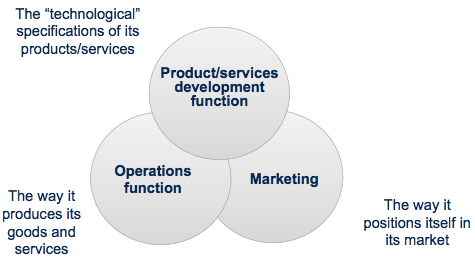
\includegraphics[width=1\textwidth]{W01/competitive_edge}
\subsubsection{Operations Can be Analyzed at Three Levels}
\index{Operations!Levels}
\index{Flow between! operations}
\index{Flow between! processes}
\index{Flow between! resources}
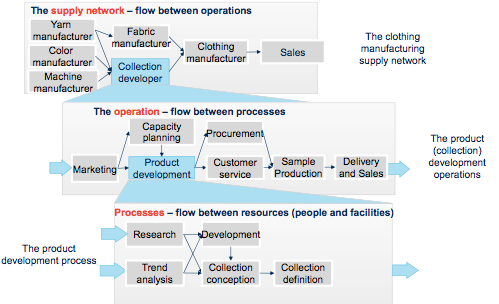
\includegraphics[width=1\textwidth]{W01/operations_three_levels}
\subsubsection{The Output of Most Types of Operation: A Mixture of Goods and Services}
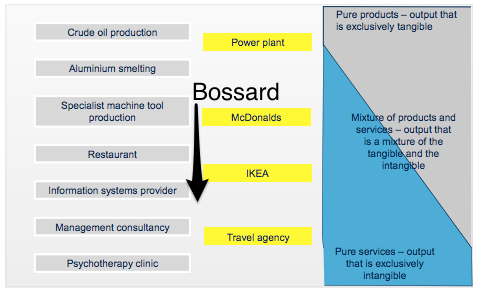
\includegraphics[width=1\textwidth]{W01/goods_and_services}
Bossard group bietet Verbindungstechnik als Dienstleistung. (Mixture  \index{Products}Products and \index{Service}Service)
\index{Pure!Products} \index{Pure!Services}
\subsubsection{Core and Supporting Processes/Functions }
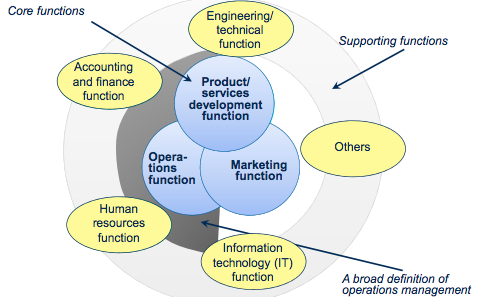
\includegraphics[width=1\textwidth]{W01/core_and_supporting_processes}
\index{Functions!Core}
\index{Functions!Supporting}

\subsection{Characteristics of OPM}
\subsubsection{Differences Within Sectors Are often Greater than the Differences between Sectors}
Aufgepasst beim Vergleich mit Branchenkennzahlen!\\
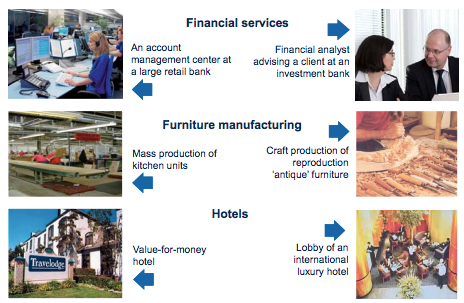
\includegraphics[width=1\textwidth]{W01/differences_betwee_sectors}
\subsubsection{The Four V’s: The Typology of Operations}
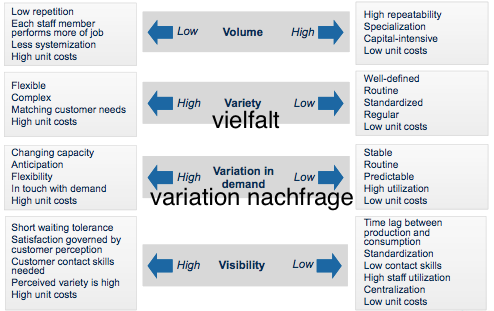
\includegraphics[width=1\textwidth]{W01/four_v}
\index{4V!Volume}
\index{4V!Variety}
\index{4V!Variation in Demand}
\index{4V!Visibility}
\subsubsection{Profiles of Different Types of Restaurants (4V)}
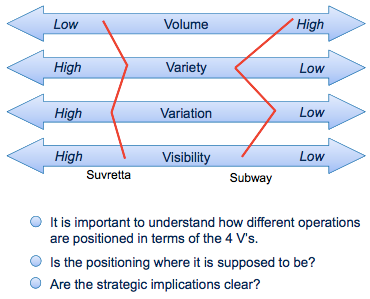
\includegraphics[width=1\textwidth]{W01/4v_restaurant}







\section{W02 - OP Strategy \& Performance}
 
\subsection{Role of Operations}
\subsubsection{The Strategic Role of Operations can be defined by its aspirations (Hayes and Wheelwright)}
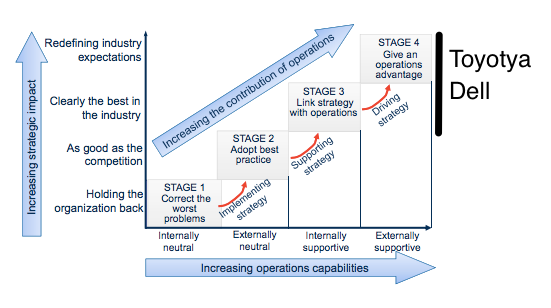
\includegraphics[width=1\textwidth]{W02/role_of_operations}
\textbf{STAGE 2 Best Practise}\\ so gut wie die anderen, nach heutigem standard. Kunde nimt einen als normalen Anbieter wahr\\
\textbf{STAGE 3: Best in Class}\\ Vorsprung wie kurze Lieferzeiten oder Preis. Kunde merkt das noch nicht.\\
\textbf{STAGE 4}\\ Nur 1 mal in der Branche. \textbf{Kunde} bemerkt Anbieter und \textbf{kommt selbst\"andig}
\index{Best in Class}
\index{Best Practice}
\index{Hayes}
\index{Wheelwright}
\subsubsection{Broad Strategic Objectives for an Operation Applied to Stakeholder Groups}
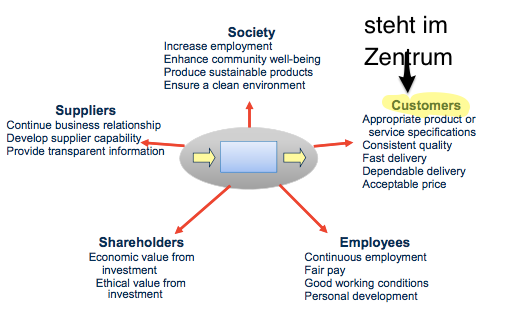
\includegraphics[width=1\textwidth]{W02/stakeholder_group}
\index{Stakeholder!Groups}
\index{Operation!Objectives}
\subsection{Operations Goals}
\subsubsection{The Five Performance Goals\index{Five Performance Goals}}\label{FivePerformanceGoals}
\index{5!Leistungsziele}
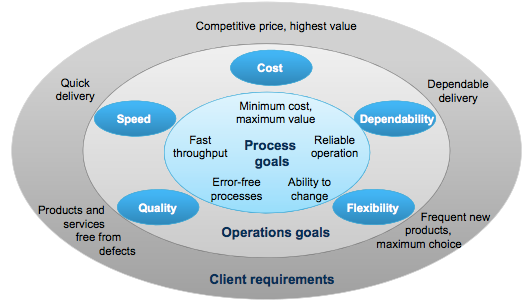
\includegraphics[width=1\textwidth]{W02/5_performance_goals}
\subsubsection{Performance Goals\index{Performance Goals} and \index{Competitive Factors}Competitive Factors}
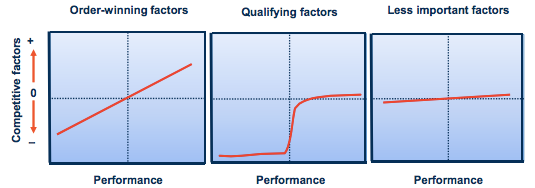
\includegraphics[width=1\textwidth]{W02/performancegoals}
\index{Factor!Order-Winning}Order-winnning factors: bei kleinen Performancever\"anderungen grosser ''Gewinn''\\
\index{Factor!Qualifying}Qualifying factors: wenn minimum nicht erreicht wird, Kunde/Auftrag verloren
\subsubsection{The Five Competitive Objectives}
\index{Competitive Objectives}
\begin{tabular}{rl}
Quality &  RIGHT\\
Speed &  FAST\\
Dependability & ON TIME\\
Flexibility & ABLE TO CHANGE\\
Cost & PRODUCTIVE\\
\end{tabular} 
= Competitivenesse\index{Competitivenesse}
\subsubsection{The Effects of the Product/Service Life Cycle on an Operation’s Performance Objectives}
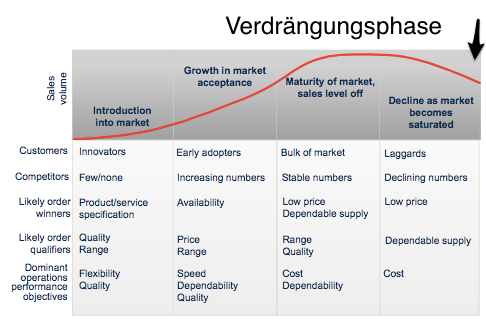
\includegraphics[width=1\textwidth]{W02/productlifecycle}
\subsubsection{Quality Means Different Things in Different Operations}
\begin{center}
\begin{tabular}{|c|c|}
	\hline Hospital & Automobile plant \\ 
	\hline Bus company & Supermarket \\ 
	\hline 
\end{tabular} 
\end{center}
\subsubsection{Cost Means Different Things in Different Operations}
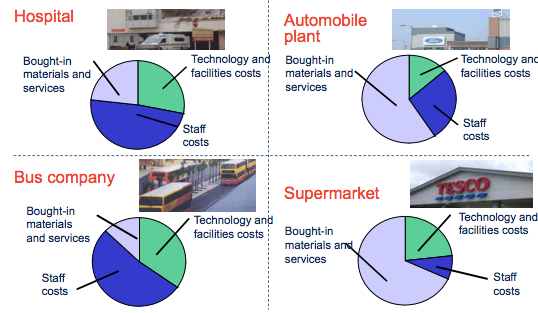
\includegraphics[width=1\textwidth]{W02/cost_operations}
\subsubsection{Polar Diagrams}
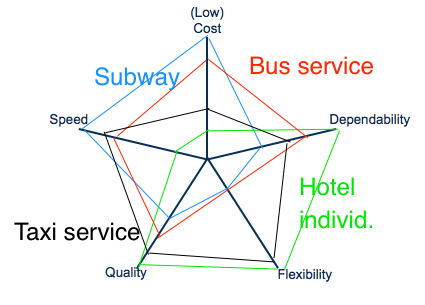
\includegraphics[width=1\textwidth]{W02/polar_diagramm}
\subsection{Strategy and Trade-Offs}
\subsubsection{What is Strategy? }\label{whatIsStrategy}
Das Kriegsche Modell\index{Kriegsche Modell}:\\
Values are fix, and mid-term goals are reacting on values.\\
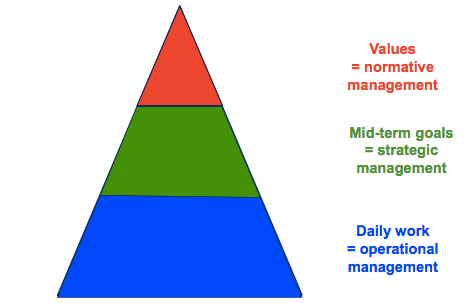
\includegraphics[width=1\textwidth]{W02/strategy}
\subsubsection{Operational Management Executes the Operations Strategy}
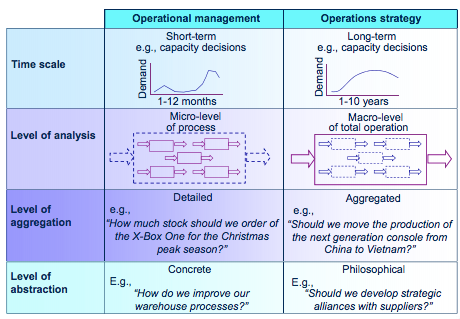
\includegraphics[width=1\textwidth]{W02/operations_strategy}
\index{Operational!Management}
\index{Operational!Strategy}
\subsubsection{The Strategic Hierarchy}
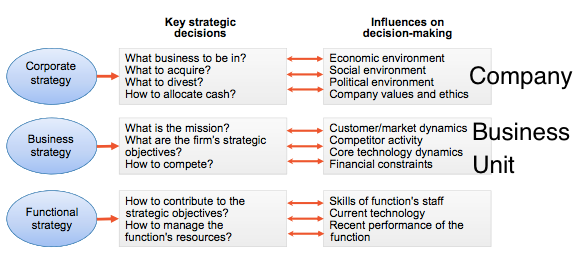
\includegraphics[width=1\textwidth]{W02/strategic_hierarchy}
\subsubsection{Mintzberg's Concept of Emergent Strategy}
\index{Mintzberg's Concept}
\index{Emergent Strategy}
\index{Strategy!Emergent}
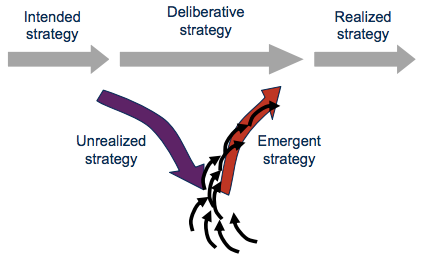
\includegraphics[width=1\textwidth]{W02/mintzberg}
\subsubsection{Good - Cheap - Fast}
Pick two :)
\subsubsection{Tradeoffs - The 'Efficient Frontier' \index{Efficient Frontier} View}
ABCD haben ''Best Practice''\index{Best Practice} erreicht, aus Sicht X ist B der gr\"osste Konkurrent.
B1 zeigt das Best in Class\index{Best in Class} ein nachhaltiger Vorteil ist.\\
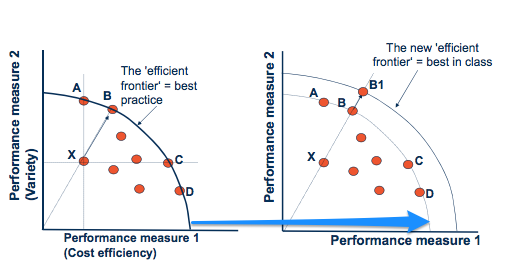
\includegraphics[width=1\textwidth]{W02/efficient_frontier}
\section{W03 - Product \& Service Design}
\subsection{Slides}
\subsubsection{The Innovation Top 20}
\index{Innovation!Top 20}
Tendenz: F\&E nach asien verlagern -> Forschung zum Markt.\\
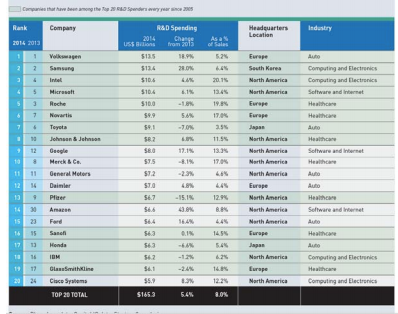
\includegraphics[width=1\textwidth]{W03/top20}
Die Autoindustrie ist gross, darum auch in den Top 20.
\subsubsection{The “Global Innovation 1000” 2014 Study: Insights}
Key take-aways
\begin{itemize}
\item The biggest 1000 companies (in R\&D volume) spent USD 647
billion on R\&D in 2014 (+/-1.4\% compared to 2013)
\item R\&D intensity on a slight decline (+0.2\%) compared to 2012 (normal 5-7\%)
\item Germany remains the biggest innovation location in Europe
\item China has increased their spending by 45.9 (was 34.4 \% in 13)
\item Strong investments in IT: Google, Samsung, Microsoft
\item Interesting newcomer: Amazon
\end{itemize}
Nur Time to Market\index{Time to Market} entscheidet, hohe TTM -> weniger Innovation
\subsubsection{Product and Service Design Activity: An Individual Process}
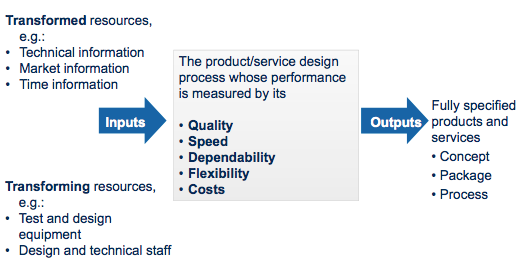
\includegraphics[width=1\textwidth]{W03/individualprocess}
\subsubsection{The Five Stages of Product\index{Five Stages of!Product} / Service Design\index{Five Stages of!Service Design}}
Floprate 50-90\%\\
\begin{center}
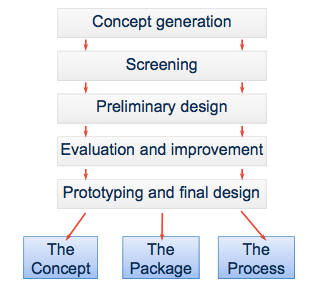
\includegraphics[width=0.5\textwidth]{W03/5stages}
\end{center}
\subsubsection{Product or Service Concept Generation}
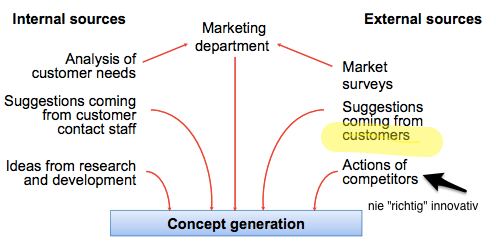
\includegraphics[width=1\textwidth]{W03/conceptgeneration}
%\subsubsection{Transforming an Idea into a Concept}
%\subsubsection{Design Involves the Process of Progressively Reducing the Number of Possibilities}
%\subsubsection{Criteria for Assessing Concepts}
%\subsubsection{Think, Try, and Experiment before You Develop!}
%\subsubsection{Early Conflict Resolution}
%\subsubsection{Where Should Management Attention Be?}
%\subsubsection{Product Structure for a Telephone}
%\subsubsection{Design for Assembly – Anticipate Operations Cost!}
%\subsubsection{Modularization and Standardization of Components}
%\subsubsection{Design to Logistics}
%\subsubsection{Prototype and Final Design}
%\subsubsection{CAD Helps in the Prototype }
\subsubsection{Time to Market\index{Time to Market} - Time Is Money}
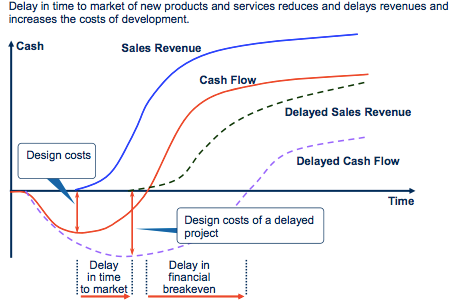
\includegraphics[width=1\textwidth]{W03/ttm}
Simultanos engineering \& Product Management
\subsubsection{Simultaneous Arrangement of the Stages in Design Activity}
\index{Concurrent!Engineering}
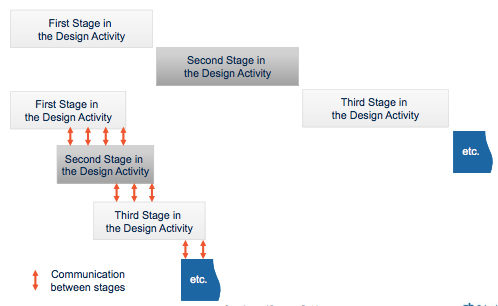
\includegraphics[width=1\textwidth]{W03/designactivity}
Parallel, this is fast but needs more flexibility!
\subsubsection{Agile Development: Scrum}
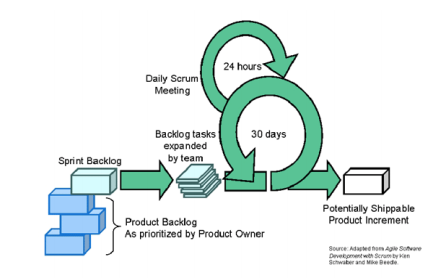
\includegraphics[width=1\textwidth]{W03/scrum}
\subsubsection{Reduction of Development Time in Aeronautics}
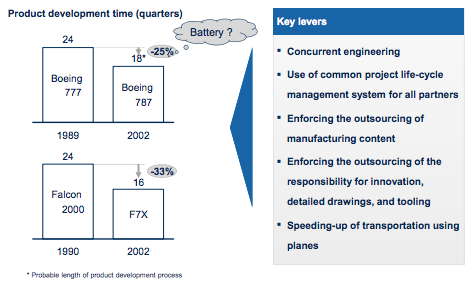
\includegraphics[width=1\textwidth]{W03/concurrent}
\section{W04 - Process Design}
 
\subsection{Process Design}
\subsubsection{Definition: (Process)Design}
\index{Design!Definition}
\begin{itemize}
\item To design is to conceive the looks, arrangement, and
workings \textbf{before} something is constructed
\item Design is therefore a \textbf{conceptual activity} that has to
deliver a solution that works in practice
\item In some languages ''design'' has a stronger connotation
with the looks of an object (artistic aspects)
\end{itemize}
\subsubsection{Designer’s Aims}
\begin{tabular}{|p{7cm}|p{7cm}|}
	\hline Product designers will seek to create things that... &  Operation managers tend to focus on the design of the tranformation process- which..\\ 
	\hline  
	are aesthetically pleasing& is flexible and efficient \\ 
	satisfy needs& supports the stategic goals of companies \\ 
	meet expcetations& is without errors \\ 
	perform well& is motivating for employees \\ 
	are reliable& is robust and easy to control \\ 
	are easy to manufacture and deliver	&  \\ 
	\hline 
\end{tabular} 
\subsubsection{Relationship between Product and Process Design}
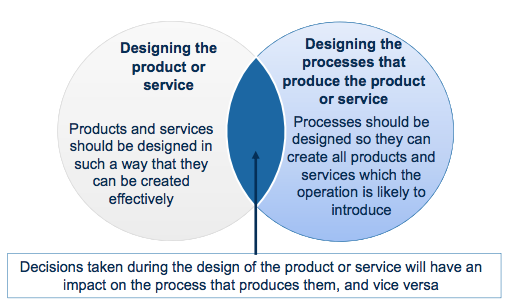
\includegraphics[width=1\textwidth]{W04/product_process_design}
\subsection{Process Types}
\subsubsection{Manufacturing Process Types\index{Process Types}}

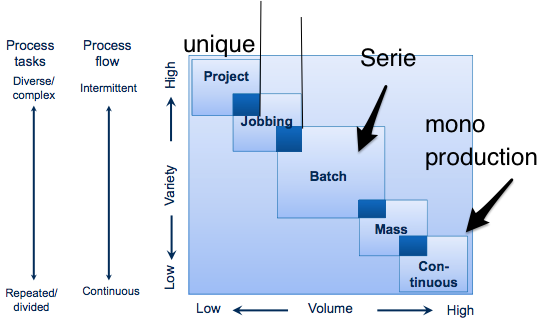
\includegraphics[width=1\textwidth]{W04/manufacturingprocesstype}
\subsubsection{Project Processes \index{Project Processes}}
\begin{itemize}
\item One-off, complex, large-scale 'products' with a
high work content
\item Defined start and finish: time, quality, and cost
objectives
\item Specially made, every one 'customized'
(engineered to order)
\item Complex planning, as many different skills have
to be coordinated
\item Fixed position layout: material is assigned to the
object
\item Examples: \textbf{Construction site}, shipyard, plant
construction
\end{itemize}
\subsubsection{Jobbing Processes\index{Jobbing Processes}}
\begin{itemize}
\item Very small quantities: 'one-offs', or only a few
required
\item Specially made: every one 'customized'
(make to order)
\item High variety and low repetition
\item Skill requirements are usually very broad
\item Skilled jobbers or team complete whole
product
\item Fixed position or functional layout
\item Examples: \textbf{Machine industry}, press cylinder,
tailor-made suits
\end{itemize}
\subsubsection{Batch Processes\index{Batch Processes}}
\begin{itemize}
\item Higher volumes and lower variety than
for jobbing
\item Standard products, repeating demand
(but can be made to order)
\item Specialized, narrower skills
\item Set-ups (changeovers) at each stage of
production
\item Functional or cell layout
\item Example: Machine tool manufacturing,
food production, clothing,\textbf{ canteen
kitchen}
\end{itemize}
50x Los am Tag produzieren / B\"acker Batch(Teig) zu Brot verarbeiten
\subsubsection{Mass Processes\index{Mass Processes}}
\begin{itemize}
\item Higher volumes than batch
\item Standard, repeat products (make to
stock) or with customer-specific
assembly (mass customization)
\item Low and/or narrow skills; high degree
of work split
\item No change-overs, or almost
instantaneous ones
\item Cell or product layout
\item Example: Automotive production,
mass electronics,\textbf{ beer bottling}
\end{itemize}
Tages-/Wochenarbeit, Automatisiert, Fluss steht im Zentrum, wenn ein Anlageteil steht so steht die ganze Produktion.
\subsubsection{Continuous Processes\index{Continuous Processes}}
\begin{itemize}
\item Extremely high volumes and low
variety:
often single product in endless flow
\item Standard, repeat products (make to
stock)
\item Highly capital-intensive and automated
\item Few change-overs required
\item Difficult and expensive to start and stop
the process, therefore few changeovers
\item Example: \textbf{petrochemical refineries},
steel-making industry, internet server
\end{itemize}

\subsubsection{\index{Process!Types}Process Types: Services }
\subsubsection{Costs of Operations}
Bsp: Beratung, wird nicht schneller mit n-Personen mehr.\\
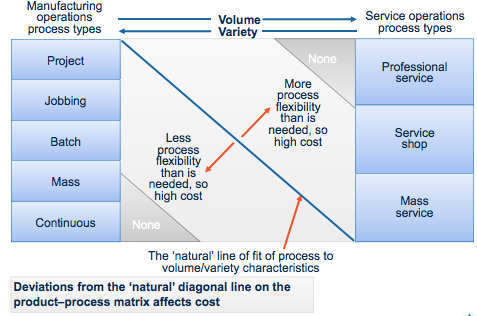
\includegraphics[width=1\textwidth]{W04/costofoperations}
\newpage
\subsection{Methods and Tools}
\subsubsection{\index{Little's Law}Little\textquotesingle{}s Law - Example }
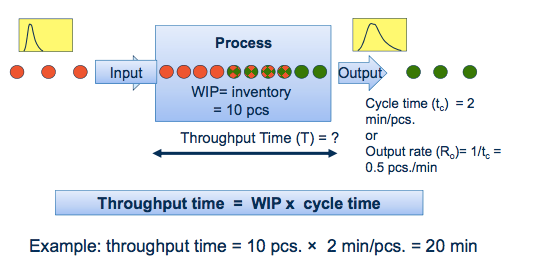
\includegraphics[width=1\textwidth]{W04/littleslaw}
\subsubsection{Little\textquotesingle{}s Law\index{Little's Law}}\label{littleslaw}
\begin{center}
	Alles in der Blackbox, egal ob in Warteschlange oder Nacharbeit, wird als Work in Progress (WIP) gez\"ahlt\\
	\begin{tabular}{|r|c|l|}
	\hline T  & Troughput time & s/min/h \\ 
	\hline WIP & Work in Progress & piece/kg/CHF \\ 
	\hline $t_c$ & cycle time & time per piece\\ 
	\hline $R_0$ & Output rate & $\frac{piece}{time}$\\
	\hline
\end{tabular}
\\\vspace{5 mm}

	$R_0$ = $\frac{1}{t_c}$ \\\vspace{2 mm}
	T =$ WIP\cdot cycle time$ \\\vspace{2 mm}
	T = $\frac{WIP}{output rate}$\\\vspace{2 mm}

\end{center}
\subsubsection{Example: Snowboarding}
\begin{center}
	120 Snowboarders ar waiting, everey 8 seconds 4 where transported.\\\vspace{2 mm}
$WIP = 120 SB $\\\vspace{2 mm}
$t_c = \frac{8 [sec]}{4[SB]} = 2[sec/SB]$ \\\vspace{2 mm}
$T = 120 [SB] \cdot 2[t_c] = 240 [sec] = 4 [min] $ \\\vspace{2 mm}
\end{center}
\subsubsection{Throughput time\index{Throughput!Time} and Processing Time\index{Processing!Time} Are not the Same!}
Nur Bearbeitungszeit ist wertsch\"opfend, Transportzeit kann auch wertsch|"opfend sein.\\
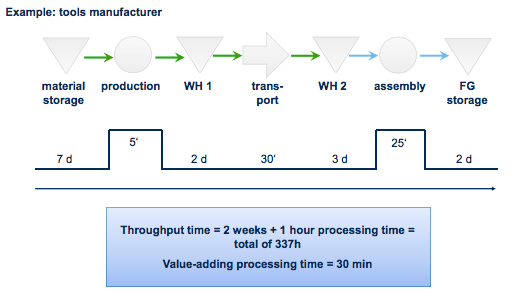
\includegraphics[width=1\textwidth]{W04/troughputvsprocessing}
\subsubsection{Little's Law Exercise: Automotive Supply Chain\index{Little’s Law}}
\begin{itemize}
\item An automotive OEM produces a new car every 2
minutes. The throughput time (from arrival of raw
materials until the car is ready for distribution) is 2
weeks. Please calculate the capital tied up in the
OEMs supply chain
\item Average value of the car during the 2 weeks of
production: CHF 20,000
\item Manufacturer's working time: 3 x 8-hour shifts on 5
days a week
\end{itemize}
\begin{center}
	
$Gebundenes Kapital minimieren \Longrightarrow schneller arbeiten$\\
$t_c = 2min =\frac{1}{30}h$\\
$T = 2w \cdot 5d \cdot 3 shifts = 240h$\\
$Bestand = 7200 Cars \cdot 20'000 = 144'000'000$\\ \vspace{2mm}
$20'000 \cdot \frac{2 \cdot 5 \cdot 24 \cdot 60}{2}=144'000'000$
\end{center}
\subsubsection{Division of Labor - Example\index{Division of Labor}}
\begin{center}
\begin{tabular}{|c|c|c|c|}
\hline Code & Activity & Predecessor & Time (min)\\ 
\hline A & Pretest  1&  - & 5\\ 
\hline B & Pretest 2 & A & 6\\ 
\hline C & De-assembly & B & 4\\ 
\hline D & Repair 1 & C & 8\\ 
\hline E & Repair 2 & C & 6\\ 
\hline F & Repair 3 & C & 4\\ 
\hline G & Assembly & D, E, F & 10\\ 
\hline
\end{tabular} 
\end{center} 
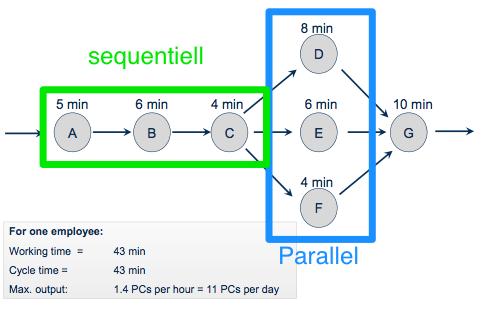
\includegraphics[width=1\textwidth]{W04/processmap}
\index{Parallel}
\index{Sequentiell}
\index{Process!Map}
\subsubsection{Division of Labor\index{Division of Labor}}
L\"angster Schritt diktiert denn Takt. \index{Balancing!Loss}Balancing Loss weil wartezeit pro Zyklus anf\"allt.\\
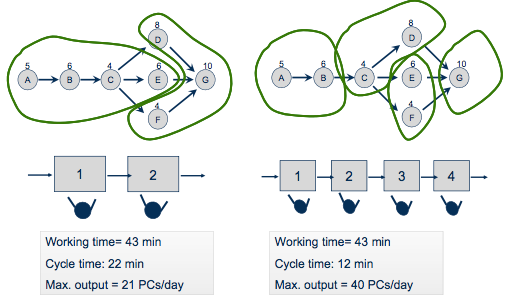
\includegraphics[width=1\textwidth]{W04/divisionoflabor}
\subsubsection{In Series (Sequentially\index{Sequentially}) or in Parallel\index{Parallel}?}
\begin{tabular}{|>{\centering\arraybackslash}p{7cm}|>{\centering\arraybackslash}p{7cm}|}
	\hline serie & parallel \\ 
	\hline kosteneffizient & robust (Ausfall) \\ 
	Erfahrungskurve (20-30\%) & flexibel(Volumen)\\
	 Weniger Platz (Infrastruktur $\cdot1$)& Variantenvielfalt
	 \\ Produktequalit\"at &   Servicequalit\"at\\ 
	\hline 
	Channeled flow, easier to manage & Higher mix flexibility \\
	Simple material handling & Higher volumen flexiblity \\
	Lower capital requirements & Higher robustness\\
	More efficient operation (higher propotion of direct productive work) & Less monotony[1]
\\
Space-saving & Greater autononmy[1] \\
	\hline
\end{tabular} 
[1] Employee motivation\\
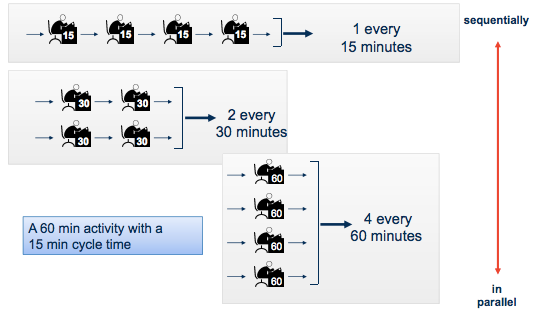
\includegraphics[width=1\textwidth]{W04/sqvspar}

\subsubsection{Balancing Processes to Avoid Loss of Efficiency}
\index{Balancing!Loss}
Verlustzeit aufgrund Arbeitsteilung, je mehr sequentiell desto h\"oher Balance Loss (Achtung Lernkurve).\\
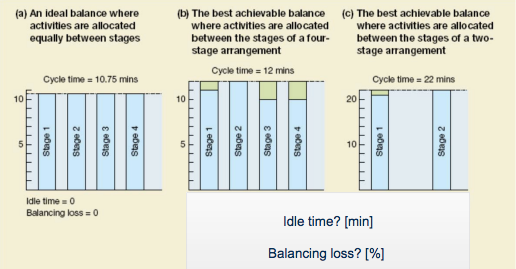
\includegraphics[width=1\textwidth]{W04/balancingprocess}
\section{W05 - Location, Layout \& Flow}
\subsection{Location of Operations\index{Location!of Operations}}
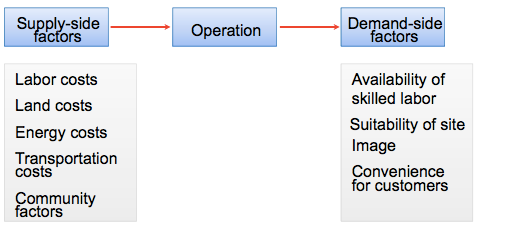
\includegraphics[width=1\textwidth]{W05/locationofoperations}
\subsubsection{Example: Cost Breakdown of Shirt Produced in Various Countries and Sold in France}
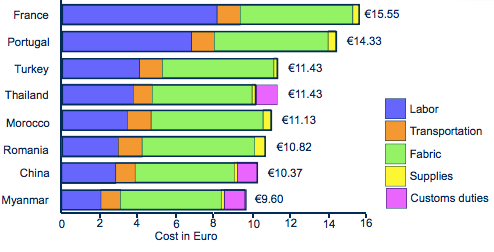
\includegraphics[width=1\textwidth]{W05/transportcost}
\subsection{Basic Layout Design\index{Layout!Design}\index{Layout}}
\subsubsection{Process Design: Design Procedure}
\index{Process!Design}
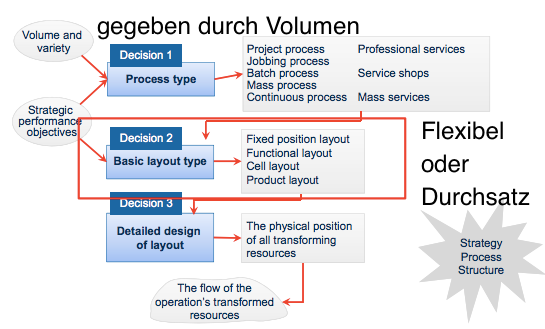
\includegraphics[width=1\textwidth]{W05/designrocess}
\subsubsection{The Nature of the Basic Layout Types}
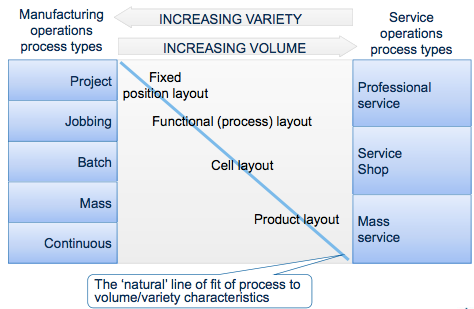
\includegraphics[width=1\textwidth]{W05/basiclayouttypes}
\subsubsection{Example of a Fixed Position Layout\index{Fixed Position Layout}: Hotel Construction Site}
Festplatz, Werft, Flugzeugbau
\begin{itemize}
\item kann nicht bewegt werden 
\item Kostenintensiv
\item Robust
\item Fixpreis -> immer mit konkretem Plan
\end{itemize}
\subsubsection{Example of  Fixed Position Layout\index{Fixed Position Layout}: Hospital OR}
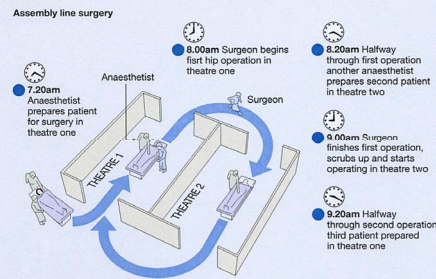
\includegraphics[width=1\textwidth]{W05/assemblylinesurgery}
\subsubsection{Example of Functional Layout\index{Functional Layout}: Glassblowing Workshop}
\subsubsection{Example of Functional Layout\index{Functional Layout}: Machine Construction}
F\"ahigkeiten werden zusammengezogen. Jegliches Produkt kann hergestellt werden. Engpass nicht Sichtbar. Lange Durchlaufszeiten.\\
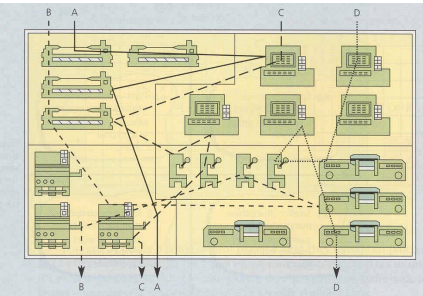
\includegraphics[width=1\textwidth]{W05/machineconstruction}
\subsubsection{Example of Functional Layout\index{Functional Layout} : Library Floor Plan}
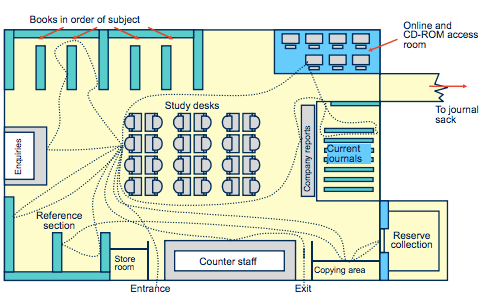
\includegraphics[width=1\textwidth]{W05/libraryfloorplan}
\subsubsection{Example of Functional Layout\index{Functional Layout} (Process): Kitchen}
\subsubsection{Example of Cell Layout\index{Cell Layout}: Machine Construction}
Flexiblit\"at nimmt ab. 5. Zelle als Werkstatt (Prototypen \& Lehrlinge). Volumen muss hoch sein. Sonst entsteht viel Leerlauf.\\
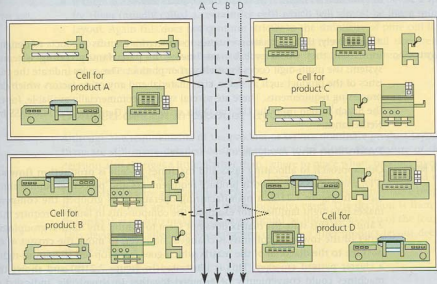
\includegraphics[width=1\textwidth]{W05/celllayoutmachine}
\subsubsection{Example of Cell Layout\index{Cell Layout}: Pharmaceutical Production}
\subsubsection{Example of Cell Layout\index{Cell Layout}: Department Store Floor Plan}
Service kann gezielt bezogen werden. Achtung, mit zentraler Kasse kein Cell Layout mehr.\\
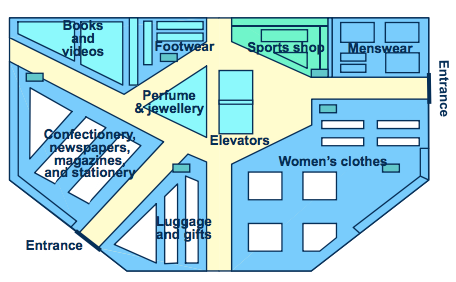
\includegraphics[width=1\textwidth]{W05/departementstore}
\subsubsection{Example of Product Layout\index{Product Layout}: Paper Production}
\subsubsection{Example of Product Layout\index{Product Layout}: Airport}
\subsubsection{Example of Product Layout\index{Product Layout}: Army Induction Center}
\subsubsection{Restaurant Using All Four Basic Layout\index{Basic Layout} Types}\label{allLayouts}
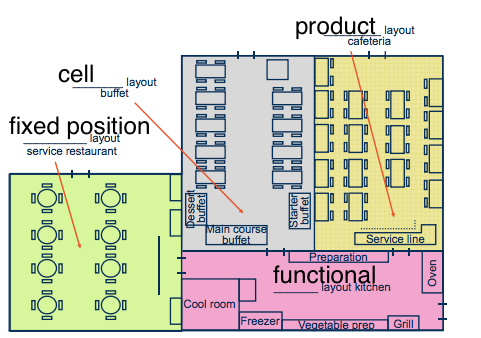
\includegraphics[width=1\textwidth]{W05/alllayouts}
\subsubsection{Revision: Basic Layout\index{Basic Layout} Types}
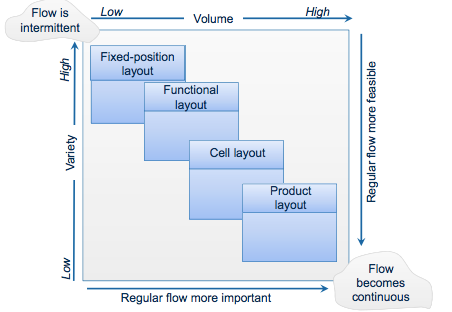
\includegraphics[width=1\textwidth]{W05/basiclayouttypesrevision}
\subsubsection{Advantages and Disadvantages}
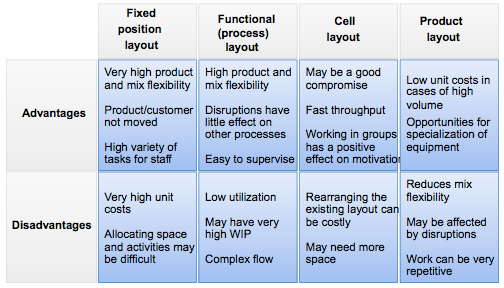
\includegraphics[width=1\textwidth]{W05/advantagesanddisadvantages}
\subsubsection{The Different Fixed and Variable Cost Characteristics Determine the Choice of Layout Type}
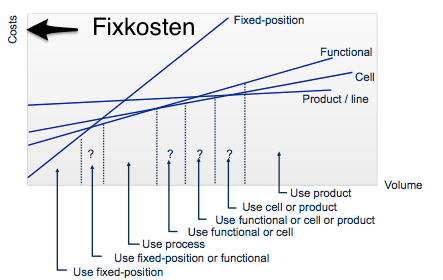
\includegraphics[width=1\textwidth]{W05/choicelayouttype}
\subsubsection{The Right Layout Type Is One Lever in Leveraging the Learning Curve}
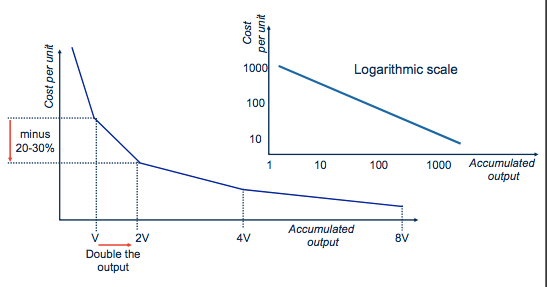
\includegraphics[width=1\textwidth]{W05/learningcurve}
\subsubsection{Examples of Learning Curve Slopes}
\includegraphics[width=1\textwidth]{W05/learningcourveslope}
\subsection{Workplace Design}
\subsubsection{The objectives of job design}
\subsubsection{Is Your Mouse Making You Ill?}
\subsubsection{Definition Ergonomics}
\subsubsection{Ergonomics: Legal Requirements}
\subsubsection{Ergonomics – How an Individual Interfaces with the Physical Aspects of His or Her Workplace}
\subsubsection{Job Design – Your Job as Manager Is to Define the Right Ergonomics for Your Team}
\begin{itemize}
\item Eliminate health riskis
\item Reduce health risks
\item Provide protection
\end{itemize}
\subsubsection{Group Exercises at the Conveyor Belt to Improve Health and Fight Burnout}
\subsubsection{Usability Engineering (Software Ergonomics)}
\subsubsection{Usability is key for a positive user experience}
\subsubsection{Basic Principles of Usability Engineering}
\subsubsection{What Is my function in an app?}
\subsubsection{Basic Principles of Usability Engineering}
\subsubsection{Usability Engineering (Software Ergonomics)}

\section{W06 - Supply Management \& Distribution}
\subsection{Supplier Network Configuration}
\subsubsection{Case Study: Dell}
\subsubsection{Market Shares until 2000}
\subsubsection{Market Shares until 2006}
\subsubsection{Market Shares today}
\subsubsection{Comparing Operating Margins}
\subsubsection{Dell's Supply Network}
\includegraphics[width=1\textwidth]{W06/dellssupplynetwork}
\subsubsection{Dell's Innovative Financing Model: Another Factor in Its Success}
\subsubsection{PC Design Evolution}
\subsubsection{Structure of Supply Networks\index{Supply!Networks}}
\includegraphics[width=1\textwidth]{W06/structureofsupplynetwork}	
\subsubsection{OperationsPerformance\index{Operations!Performance}: A Whole Supply Chain \index{Supply!Chain}Issue}
Benefits of looking at the whole supply chain include:
\begin{itemize}
	\item It puts the operation into its competitive context
	\item It helps to identify the keay players
	\item It shifts emphasis to the long term
	item It sensitizes the operation to macro-changes
\end{itemize}
\includegraphics[width=1\textwidth]{W06/supplychainissue}	
\subsubsection{Supply Network\index{Supply!Network} Design: Extension of Process Span}
Example for horizontal integration: google into car production (not in the own supply chain). \\ \index{Integration!horizontal} \index{Upstream!vertical Integration}
\index{Downstream!vertical Integration}
\includegraphics[width=1\textwidth]{W06/extensionofprocessspan}	
\subsubsection{The Decision Logic of Outsourcing\index{Outsourcing}}
Know How strategisch -> kein Outsourcing
Outsourcing nur aus Kostengr\"unden ist nicht Lohnenswert.\\
\includegraphics[width=1\textwidth]{W06/outsourcing1}
\subsubsection{Relationship between Offshoring\index{Offshoring} and Outsourcing\index{Outsourcing}}
\begin{center}
\includegraphics[width=0.5\textwidth]{W06/outsourcingvsoffshoring}
\end{center}

\subsubsection{Trends in Outsourcing\index{Outsourcing} Example: Automotive Industry}
Percentage of in-house value creation of German automotive OEM\index{OEM}s - Wertsch\"opfung = Kosten + Marge? \\
\includegraphics[width=1\textwidth]{W06/autooem}
\subsection{Supplier Management}
\subsubsection{The complexity of \index{Supplier Management} forces an systematic approach – Example Metro Germany}
\subsubsection{A material classificaiton is the basis for a segmented approach towards suppliers}
\includegraphics[width=1\textwidth]{W06/classification}
\subsubsection{How to segment your supplier – Example scorecard}
\subsubsection{Supplier Management\index{Supplier Management}: Measure and score their performanceregularly}
\subsubsection{An ambitious route of managing suppliers: Develop them further – example Toyota}
\subsection{Distribution\index{Distribution}}
\subsubsection{Distribution\index{Distribution}: From the Manufacturer to the Stores}
\subsubsection{Distribution\index{Distribution} and Channels\index{Channels}}
\includegraphics[width=1\textwidth]{W06/distributionandchannels}
\subsubsection{Transportation of Materials: Key Figures for Switzerland}
\subsubsection{Distribution: Example of Swiss Retailer}
\subsubsection{Cross-Docking\index{Cross-Docking}: Modern Distribution\index{Distribution} System}
Nichts mehr einlagern, nur kurz zwischenlagern, fixer \& schneller. Verteilzentren werden aufgel\"ost.\\
\includegraphics[width=1\textwidth]{W06/crossdocking}
\subsubsection{Indirect distribution costs are often overlooked}
3) zu viel an Lager\\
6) zu wenig an Lager\\
\includegraphics[width=1\textwidth]{W06/indirectcosts}
\section{Presentations}
\subsection{Coop at Home}
\subsection{admin}
\section{W08 - Supply Chain Management}
\subsection{Introduction to SCM \index{Supply Chain Management}}
\subsubsection{The Revolution in 1983}
\subsubsection{Swatch 1992: 100’000’000 Uhr }
\subsubsection{Understanding the Impact of Supply Chain Disruptions}
\subsubsection{Supply Chain Glitches\index{Supply Chain!Glitch} Can Affect a Company’s Performance}
Auswirkung auf Aktienkurs be Lieferproblemen, x-Achse = 1 Jahr.\\
\includegraphics[width=1\textwidth]{W08/glitch}
\subsubsection{Comparison: The Effect of a Supply Chain Glitch	(-20\% to -25\% Stock Price Reduction)}
\begin{tabular}{|l|l|}
	\hline Statement & Stock Price Reaction \\ 
	\hline \multicolumn{2}{|c|}{ \textbf{Operations Events}}   \\ 
	\hline Increase in R\&D spending & 1.4\% \\ 
	\hline Closing factories & -0.7\% \\ 
	\hline Successful TQM & 0.6\%  \\ 
	\hline Successful green initiatives & 1.9\%  \\ 
	\hline  \multicolumn{2}{|c|}{ \textbf{Marketing Events}}    \\ 
	\hline Contracting of celebrities & 0.2\%  \\ 
	\hline Introduction of new product & 0.3\%  \\ 
	\hline  \multicolumn{2}{|c|}{ \textbf{IT}}    \\
	\hline  IT problems & -1.8\%  \\ 
	\hline 
\end{tabular} 
\subsubsection{Case Study: McDonalds Meat Scandal in China}
\subsubsection{Case Study: Toyota}
\subsubsection{Was Everything just a Misunderstanding? }
\subsubsection{Which Industries Are most Likely to Be Influenced by Supply Chain Glitches?}
\subsubsection{Supply Chain Management\index{Supply Chain!Management}:	From Sheep to Shawl}
\subsubsection{This is not Supply Chain Management – Optimizing yourself on	cost of other players in the chain}
! Just in Time  ist gef\"ahrlich!
spezialisierte Produkte die schnell ausgeliefert werden m\"ussen, brauchen hohe Lagerkosten. Auf keinen Fall zum externen Warenlager werden.
\subsubsection{Logistics = Supply Chain Management ?}
\subsubsection{Key Terminology of Supply Chain Management}
\includegraphics[width=1\textwidth]{W08/keyterm}
\subsection{Bullwhip Effect}
\subsubsection{The Bullwhip Effect: Increasing Variability Upstream\index{Upstream}}
1. F\"ur den Bullwhip Effect\index{Bullwhip!Effect} braucht es ''st\"orung'' in der Beschaffung (mehr Einkauf als geplant)\\
2. F\"ur Bullwhip Effect braucht es einen Zeitverzug zwischen Suppliers.
Um zu vermeiden -> alle in der Lieferkette m\"ussen informiert sein.
\includegraphics[width=1\textwidth]{W08/variabilityupstream}
\subsubsection{The Bullwhip Effect Can also Happen within a Company}
\subsubsection{Even Whole Economies Can Become Volatile: Machine Tools at the Tip of the Bullwhip}
\subsubsection{The Bullwhip Effect during the Financial Crisis in 2009}
\subsubsection{Impact of Bullwhip}
\index{Bullwhip!Impact}
\begin{enumerate}
\item High inventory
\item Out-of-stocks (OOS\index{OOS}) backlog cost
\item Low operational efficiency
\begin{itemize}
	\item underutilization
	\item overtime
	\item expediting
	\end{itemize}
\item Unnecessary capacity investment
\item Swings in working capital
\end{enumerate}
\subsubsection{What causes the Bullwhip Effect? 6 Main Reasons}
\begin{enumerate}
	\item Over-reaction to backlogs
	\item Neglecting to order based on inventory position
	\item Ordering in batches 
	\item Price variations (eq. Promotions)
	\item Lack of communication \& coordination - shortage gaming
	\item Delay times for information and delivery of materials
\item
\end{enumerate}
\subsubsection{Reducing the Price (Promotions) Creates Spikes}
\includegraphics[width=1\textwidth]{W08/bullwhipnoodlesoup}
\subsubsection{``Chinese Whispers``: Information Distortion along the Supply Chain}
If one start to panic, all will start to panic. -> Domino
\subsubsection{How to Fight the Bullwhip Effect?}
\begin{enumerate}
	\item ERP-Systeme
	\item SCM-Systeme
	\item konstante Preise
	\item automatisierter Datenaustausch
	\item E-Commerce
	\item Vendor Managed Inventory
	\item automatisierte Bestellsysteme
\end{enumerate}
\subsubsection{ Automatic Replenishment Systems Can Mitigate the Effects of Overreaction}
\subsubsection{Eliminate Promotions with ``Every Day Low Prices`` (EDLP)}
\subsubsection{Handelsradar (Mai 2011) – Datenaustausch zwischen Industrie und Handel}
\subsubsection{Handelsradar Supply Side: Warum tauschen Sie nicht mehr	Daten aus?}
\subsubsection{Shorten Supply Chain: Let the Vendor Manage the Inventory}
\subsection{Designing the Supply Chain}
\subsubsection{Goals of Supply Chain Management}
\begin{itemize}
	\item Right quality: Every link is responsible for its own quality and that of its suppliers 
	\item High speed: The faster the throughput time, the more flexible	and cheaper the whole chain becomes 
	\item Reliability: Being on time, in full deliveries on all supply chain tiers 
	\item Flexibility: Supply chain agility is a prerequisite for reacting effectively to glitches and changes
	\item Cost: Reducing the overall transaction and transport costs of the whole chain
\end{itemize}
\subsubsection{How to design and optimize a Supply Network?}
\subsubsection{Choose the Right Supply Chain for each Product: Segmentation Logic by M. Fisher}
\subsubsection{Different Products Require Different Supply Chain Strategies}

\section{W09 - Capacity Management}
\subsection{Introduction}
\subsubsection{What Capacity Does this Operation Have?}
\subsubsection{What is Capacity? }
\begin{itemize}
	\item Capacity is in the static, physical sense the fixed volume of a container,
	or the space in a building, or the seats in a plane, theater, etc.
	\item The definition of the capacity of an operation is the maximum level of
	value-added activity over a period of time that the process can achieve
	under normal operating conditions
\end{itemize}
\subsubsection{Capacity Constraints}
\begin{itemize}
	\item The parts of the operation that are operating at their capacity ‘ceiling’
	are capacity constraints for the whole operation.
	\item These constraints are often referred to as ‘bottlenecks’. Depending on
	the nature of demand, different parts of an operation may be pushed to
	their capacity ceiling and act as a bottleneck.
\end{itemize}
\subsubsection{Capacity Metaphor }
\subsubsection{Medium- and Short-Term Capacity Planning}
Medium-term capacity planning involves an
assessment of demand forecasts over a period of 2 to
18 months, during which time planned output can be
varied, for example, by changing the number of hours
the equipment is used \\
Short-term capacity planning adjusts the resources
with a time horizon of days or hours, e.g. the services
in a garden restaurant
\subsubsection{Basic Questions in Capacity Planning}
\begin{itemize}
	\item Demand quantity
	\item Dependencies of the demand
	\item Demand seasonality 
	\item Limits of supply 
	\item Storing capabilities of offered product 
	\item Available capabilities
\end{itemize}
\subsubsection{Good forecasts are essential for effective capacity planning}
\subsubsection{Causes of Seasonality}
\subsubsection{Demand Fluctuation Hotel}
\subsubsection{Demand Fluctuation Retailer}
\subsubsection{Demand Fluctuation Aluminium manufacturer}
\subsection{Planning Capacity}
\subsubsection{Ways of Reconciling Capacity and Demand}
\subsubsection{Level Capacity Plan with Inventory Built up}
\subsubsection{Chase Demand Plan}
\subsubsection{Adjust Personnel Resources to Match Demand}
\subsubsection{Combination of Different Capacity Planning Strategies}
\subsubsection{Create a Capacity Plan: Cumulative Demand}
\subsubsection{Create a Capacity Plan: Cumulative Demand}
\subsubsection{Cumulative Representations: Level Capacity Plan}
\subsubsection{Cumulative Representations: Level Capacity Plan, Starting without an Inventory}
\subsubsection{Cumulative Representations: Level Capacity Plan, Starting with an Inventory}
\subsubsection{Cumulative Representations: Chase Demand Plan, Starting with an Inventory}
\subsubsection{Exercise: Capacity Planning}
\subsubsection{Challenge: The Balance of Capacity}
\subsubsection{Capacity-Leading or -Lagging Strategies}
\subsubsection{Small or Big Lots?}
\subsection{Capacity and Queues}
\subsubsection{Simple queuing system}
\subsubsection{Simple Queuing System (Continued)}
\subsubsection{Capacity vs. Lead-Time}\subsubsection{Goal: Reduce the Variance of the System }

\section{W10 - Inventory Management}
\subsection{Introduction}
\subsubsection{Water Consumption During the 2006 World Cup Championship}
\subsubsection{Visual Interpretation of Inventories}
\subsubsection{What other reasons are there for holding inventories?}
\subsubsection{Case Study: Leaving Everything Behind…}
\subsubsection{The Strategic Role of the Inventory: The Five Operations Performance Objectives}
\index{Operations!Performance Objectives}
Bsp: Zementfabrik, lange Anlaufzeit.\\
Ersatzteile, Kundennachfrage\\
cost -> Aktionen / Rabatte \\
\begin{itemize}
	\item Supporting \textbf{quality} objectives
	\item Supporting \textbf{speed} objectives
	\item Supporting \textbf{dependability} objectives
	\item Supporting \textbf{flexibility} objectives
	\item Supporting \textbf{cost} objectives
\end{itemize}
\subsubsection{Types of Inventory}
\begin{itemize}
	\item Buffer (NORDAL)
	\item Cycle
	\item De-coupling (Serielle Produktion (0.6*0.9))
	\item Anticipation (Gleichm\"assige Produktion, Absatz in kurzer frist, ex: Osterhasen)
	\item Pipeline (Lager w\"ahrend Transport)
\end{itemize}
\subsubsection{Disadvantages of Holding Inventory}
\begin{itemize}
	\item May become \textbf{obsolete} as alternatives become available
	\item Can be \textbf{damaged} or deteriorate
	\item Could be \textbf{totally lost},or be very expensive
	to retrieve
	\item Might be \textbf{hazardous} to store
	\item May need excessive \textbf{storage space} compared to its value
	\item If \textbf{duplicated} at different locations, it may be reordered at one
	location while excess inventory exists at others
	\item Involves high \textbf{administrative} and \textbf{insurance} costs
\end{itemize}
\subsubsection{Typical Inventory Profiles}
\subsubsection{The 3 Main Questions of Inventory Management}
\begin{itemize}
	\item \textbf{How much} should I order? (Q)
	\item \textbf{When} should I order? ($\frac{Q}{D}$)
	\item How should I \textbf{control the system}?
\end{itemize}
\subsection{Reordering Approach}
\subsubsection{Reducing the Reorder Quantity Reduces Stock While Increasing the Reorder Frequency}
\includegraphics[width=1\textwidth]{W10/reducingreorder}
\subsubsection{Trade-Offs in Considering Optimal Quantity}
\subsubsection{EOQ\index{EOQ}: Economic Order Quantity (based on simplified assumptions)}
\includegraphics[width=1\textwidth]{W10/EOQ-simplyfied}
\subsubsection{How to Calculate the Economic Order Quantity }\label{EOQ}
\begin{center}
\begin{tabular}{|c|c|}
	\hline Holding Costs  & Order Costs \\ 
	\hline Working capital costs & Cost of placing an order \\
	Storage costs \& Price discount costs\\
	Obsolescence risk costs & \\
	\hline
\end{tabular}
\\\vspace{5 mm}
	\begin{tabular}{|r|l|}
		\hline EOQ  & Minimal total costs \\ 
		\hline Q  & Ordering quantity \\ 
		\hline $C_t$ & Total sourcing costs \\ 
		\hline $C_O$ & ordering costs per order\\ 
		\hline $D$ & Demand per Period$t_p$\\
		\hline $S$ & Safety Stock\\
		\hline $C_h$& Holding costs per unit ($t_p$)\\
		\hline
	\end{tabular}
	\\\vspace{5 mm}
	
	$C_h$ = $\frac{C_h\cdot Q}{2 + C_h \cdot S}$\\\vspace{2mm}
	$C_O$ = $\frac{C_O \cdot D}{Q}$\\\vspace{2mm}
	$C_t$ =  $C_h + C_O$\\\vspace{2mm}
	$EOQ = \frac{D \cdot C_t}{D \cdot Q} = 0$ \\\vspace{2 mm}
	$EOQ = \sqrt{\frac{2 \cdot C_O \cdot D}{C_h}}$ \\\vspace{2 mm}
	Order frequency = $\frac{D}{EOQ}$\\\vspace{2mm}
	Time between orders = $\frac{EOQ}{D}$\\\vspace{2mm}
	
\end{center}
\subsubsection{Exercise – determining the EOQ for our motors}

\subsubsection{The Total Costs Are Relatively Unaffected by Q}
\subsubsection{Reorder Point Method}
\subsubsection{Safety Stock Required to Cover Excessive Demand and/or Delivery Insecurity}
\subsubsection{How to Calculate the Safety Stock? Example: A Bar}
\subsubsection{Safety Stock and Remaining Risk: Demand and Delivery Lead Time are Statistic Distributions Frequency}
\subsubsection{Inventory Costs vs. Availability}
\subsection{Inventory Control}
\subsubsection{Pareto Curve for Stocked Items (ABC Analysis)}
\subsubsection{Inventory Classifications and Measures}
\subsubsection{Example: Pareto Distribution for a Pharmaceutical Co. A long tail of SKUs representing only a small part of the overall volume }

\section{W11 - Planning \& Control Activities}
\subsection{Planning and Control}
\subsubsection{Planning or Control?}
\subsubsection{Definitions}
\subsubsection{Example: Air France Flight Plan: What Do You Have to Plan?}
\subsubsection{Example: SWISS: European Airbus Fleet Flight Plan for one Day }
\subsubsection{Significance of Planning and Control Time horizon Hours/days Days/weeks/months Months/years}
\subsubsection{Dependent and Independent Demand }
\subsubsection{The Order Penetration Point (OPP)}
\subsubsection{Goals to Optimize with the OPP}
\subsection{The 4 Main Activities of P\&C}
\subsubsection{The Activities of Planning and Control}
\subsubsection{Scheduling Using a Gantt Diagram}
\subsubsection{Factors Affecting Operating Time}
\subsubsection{Finite and Infinite Loading of Work Centers}
\index{Loading!Finite}
\index{Loading!Infinite}
\includegraphics[width=1\textwidth]{W11/finitevsinfinite}
\subsubsection{Local Decision Rules\index{Local Decision Rules}, e.g., Sequencing}
4 jobs for 1 work center may be planned according to the following possibilities:
$4 \cdot 3 \cdot 2 \cdot 1 = 24 possibilities$

n jobs for 1 work center yields $n!$ possibilites of sequencing\index{sequencing}\\
n jobs for m work centres yields $n^m$ possibilities of sequencing.
\subsubsection{Sequencing: Minimizing Throughput Time}
\subsubsection{Gantt Diagram of Your Orders}
\subsubsection{Planning Boards: Visible Communication Tool for Use Between Planning and Production and within Production}
\subsection{Enterprise Resource Planning}
\subsubsection{ERP = Enterprise Resource Planning}
\subsubsection{The Development of ERP}
\subsubsection{Material Requirements Planning (MRP)}
\subsubsection{Total Future Demand Is Made up of Known and Forecast Demand}
\subsubsection{Example: Treasure Hunt Game Product Structure}
\subsubsection{‘Treasure Hunt Game’: Indented Bill of Material}
\subsubsection{ERP Structure for a Sandwich Company}

\section{W12 - Lean Synchronization}
\subsection{History of Lean }
\subsubsection{Lean Management and Just in Time (JIT)}
For Slack et al., the following terms are synonymous
\begin{itemize}
	\item continuous flow manufacture
	\item high value-added manufacture
	\item stockless production
	\item low-inventory production
	\item fast-throughput manufacturing
	\item lean manufacturing
	\item Toyota production system
	\item short cycle-time manufacturing
\end{itemize}
\subsubsection{Toyota Simultaneously Increases Quality and Productivity}
\subsubsection{Introductory Movie on Lean }
\subsubsection{JIT Definitions}
\subsubsection{Lean Optimizes 3 Aspects Simultaneously}
\subsubsection{Successful lean projects are based on 3 preconditions}
\subsection{3 Value Destroyers}
\subsubsection{The 3 Value Destroyers: Waste, Variability, and Inflexibility }
\subsubsection{The 7+1 Types of Waste (= muda\index{muda})}
\begin{enumerate}
\item overproduction
\item waiting time
\item transport
\item over-process/poor process
\item inventory
\item motion
\item defective gooods
\item \textit{people's unused potential}
\end{enumerate}
\subsubsection{There Is a Gray Area Between Waste and Value-Added Activity}
\subsubsection{Variability: 5 Typical Reasons}
\begin{itemize}
\item Enviroment
\item People
\item Process/Tools
\item Material
\item Information
\end{itemize}
\subsubsection{Inflexibility: We Are Used to Waste}
\subsection{The Lean Toolbox}
\subsubsection{How to Become Lean – Example of a Toolset}
\begin{enumerate}
	\item Analyze processes
	\item Reduce inventories 
	\item Optimize process technology
	\item Standardize
	\item Change over quickly (SMED)
	\item Implement flow/ level	scheduling (Heijunka\index{Heijunka})
\end{enumerate}
\subsubsection{ There Are 3 Types of Processes}
\begin{enumerate}
	\item What the process really is
	\item What we think the process is
	\item What the process should be
\end{enumerate}
\subsubsection{Airbus A340-300 Maintenance Services}
\subsubsection{Spaghetti Diagrams}
\subsubsection{Reducing Waste}
\subsubsection{Spaghetti Diagram in a Hospital:	Preparing the Surgical Carts for the OR}
\subsubsection{ The Problem with Inventory}
\subsubsection{ Process Technology (Small-Scale Technology)}
\subsubsection{ Example of Standardized Work}
\subsubsection{Definition of Standardized Work\index{Standardized!Work}}
Standardized work is the currently best way to safely complete an activity with the proper outcome and the highest quality
\subsubsection{How Pit Stop Teams Manage Their Fast	Tire Changes?}
\subsubsection{Reducing Set-Up Reduces Inventory: SMED – Single Minute Exchange of Die}
D=demand\\
$C_O$ = ordering (set-up) cost = \textsterling
400 / order\\
$C_h$ = holding cost = \textsterling
900 / item / yr = \textsterling
900\\
Eonomic order quantity (EOQ\index{EOQ}):\\
$\sqrt{\frac{2 \cdot D \cdot C_O}{C_h}}$ = $\sqrt{\frac{2 \cdot 5000 \cdot 400}{900}}$ = 67 \\
Reducing the order (set-up) cost from \textsterling
400 to \textsterling
100:\\
$\sqrt{\frac{2 \cdot 5000 \cdot 100}{900}}$ = 33.33\\
\textbf{SMED}\\
Single minute exchange of die ist eine Messgr\"osse wie lange man zur Umr\"ustung einer Maschine braucht vom letzten produzieren Teil bis zum ersten neuen
\subsubsection{Levelled Scheduling (Heijunka\index{Heijunka}) Balances the Mix of Products Produced every Day}
Der Mix und das Volumen zwischen versch. Stationen soll gleich behalten werden. Das f\"uhrt zu kleinere Menge die verschoben werden m\"ussen, kleinere Lager n\"otig, Fehler werden schneller aufgedeckt, einfachere Planung
\subsubsection{Levelled Scheduling (Heijunka\index{Heijunka}) Balances the Mix of Products Produced every Day (Continued)}
\subsubsection{Delivering Smaller quantities More Frequently Can Reduce Inventory Levels}
\subsubsection{Basics of Material Flow: Credo of Lean Production}
\index{Lean!Production Credo}
Eliminate the \textbf{U}nnecessary -> \textbf{S}implify the necessary -> \textbf{A}utomate Simplified processes = \textbf{''USA\index{USA}''}
\subsubsection{How to Become Lean – Example of a Toolset }\label{sssec:becomelean}
\begin{enumerate}
	\item Analyze processes
	\item Reduce inventories
	\item Optimize process technology
	\item Standardize
	\item Change over quickly (SMED)
	\item Implement flow/ level scheduling (Heijunka)
\end{enumerate}
\subsubsection{Read More on Lean Banking on Moodle…}
\subsubsection{The 3 Step Approach to Lean Banking}
\begin{enumerate}
	\item Identify \textbf{customer needs}
	\item Understand \textbf{root causes} for poor performance
\item Create \textbf{behavioral change}
\end{enumerate}
\subsubsection{Poor Performance – Examples of Wastes in a Mortgage Process (Muda\index{Muda})}
\includegraphics[width=1\textwidth]{W12/poorperformance}
\subsubsection{How to Achieve the Transformation? Use your Operations	Knowledge – Example Capacity}
\subsubsection{Lean Banking Can Transform Every Part of a Bank}

\section{W13 - Quality Management}
\subsubsection{Repetition: The 7+1 Types of Waste (= muda)}
\subsubsection{Revision: How to Become Lean – Example of Toolset }
\ref{sssec:becomelean}
\subsection{Quality and Errors}
\subsubsection{What is Quality in Production? }
\subsubsection{What is Quality in Service?}
\subsubsection{Revision: Quality means different things in different operations}
\subsubsection{Perceived Quality is Governed by the Gap Between Customers’ Expectations and Their Perceptions of the Product or Service}
\subsubsection{High Quality Puts Costs down and Revenue up}
\subsubsection{A ‘Gap’ Model of Quality}
\subsubsection{The Perception – Expectation Gap}
\subsubsection{Conformance to Specification}
\subsubsection{Quality Characteristics of Goods and Services}
\subsubsection{Quality Problem – Whose Fault Was It? }
\subsubsection{Why Examine and Change Processes? Among Other Things, to Increase Quality and Reduce Errors}
''The majority of (medical) errors do not result from
individual recklessness or the actions of a particular
group - this is not a ''bad apple`` problem.
More commonly, errors are caused by faulty systems,
processes, and conditions that lead people to make
mistakes or fail to prevent them''
\subsubsection{What is the Magnitude of Errors? }
Typical range of cost of poor quality
(COPQ as \% of Sales):\\
\begin{center}
\begin{tabular}{|l|r|}
	\hline Manufacturing & 20-30\% \\ 
	\hline Services & 30-40\% \\ 
	\hline Software & 40-65\% \\ 
	\hline 
\end{tabular} 
\end{center}
\subsubsection{TQM Can be Viewed as a Natural Extension of Earlier Approaches to Quality Management}
\subsubsection{Total Quality Management: What Does TQM Include?}
1. Includes all parts of the organization
2. Includes all staff of the organization
3. Includes consideration of all costs
4. Includes every opportunity to get things right
5. Includes all the systems that affect quality
6. And it never stops!
\subsubsection{The Internal Customer–Supplier Concept Involves Understanding the Relationship Between Processes}
\subsubsection{The Traditional Cost-of-Quality Model}
\subsubsection{The Traditional Cost-of-Quality Model with Adjustments to Reflect Criticism of TQM}
\subsubsection{How to Prevent Errors Cheaply: Poka-Yoke}
-> Idiotensicher
\subsubsection{Poka-Yoke or Bullet-Proof Assembly for Kite Surfers}
\subsubsection{Poka-Yoke is a Japanese Term Meaning ''Fail-Safing'' or ''Mistake-Proofing'' }
\subsubsection{Increasing the Effort Spent on Preventing Errors from Occurring in the First Place Leads to a more than Equivalent Reduction in other	Cost Categories}
\subsubsection{The Cost of Rectifying Errors increases the Longer the Errors Remain Uncorrected in the Development and Launch Process}
\subsubsection{TQM in Services}
\subsubsection{How to Assure Quality in Services? TQM at UPS}
\subsubsection{How to Measure and Prove Quality? Examples of Certification and International Codes }
\subsubsection{EFQM ‘Business excellence’ Model}
\subsubsection{EFQM Characteristics }
Self assessment (it’s possible to adapt weighting system
of the 9 categories)
Excellent results can only be achieved if the interests of all
involved parties are taken into account
Methods: benchmarking, Kaizen, PDCA Cycle, etc.
''Committed to Excellence'': 3 successful implemented
improvement concepts and audit through validator (2-year
shelf life)
''Recognized to Excellence'': Extensive self assessment and
audit; ''Stars Award'' depending on points achieved
Competition in Switzerland: ESPRIX – Swiss Excellence
Award
\subsection{Quality Assurance}
\subsubsection{Quality Management in Daily Life: Wasabi-nuts}
\subsubsection{Costs of Poor Performance / Quality}
\begin{itemize}
	\item \textbf{Defects}\index{Defects} any instance when a proces fails to satisfy ist customer
	\item \textbf{Prevention costs}\index{Prevention costs} are associate with preventing defects before they happen
	\item \textbf{Appraisal costs}\index{Appraisal costs} are incurred when the firm assesses the performance level of the processes
	\item \textbf{Internal failure costs}\index{Internal failure costs}, result from defects that are discovered during production of a service or products
	\item \textbf{External failure costs}\index{External failure costs}, arise when a defect is discovered after the customer receives the service or product
\item
\end{itemize}
\subsubsection{Important Analytical QA Methods: QA Instruments in Practice }
\subsubsection{SPC - Natural vs. assignable causes of variation}
\subsubsection{Natural Variations vs. Assignable Variations}
\subsubsection{Histogram: Standard Deviation = Measure for Deviation}
\subsection{Six Sigma}
\subsubsection{Six Sigma: Basic Information}
\subsubsection{Process Variation and Its Effect on Process Defects per Million Opportunities (DPMO)}
\subsubsection{Low Process Variation Allows Changes in Process Performance to be Readily Detected}
\subsubsection{Six Sigma is Based on 3 Main Elements}
\section{Berechnung OEE / OPE (Alle Wege)}
\subsection{OEE: Unterscheidung Sequentiell und Parallel}
\section{OPE}
Zusammenhang OPE Zykluszeit \& Balancing Loss (Balancing Loss ist auf Basis ist Zykluszeit und nicht Kapazit\"aten)
\ref{balancingLoss} Berechnung Balancing loss
\section{Heijunka -> Unterscheidung Heijunka viele Maschinen und nur eine Maschine}
http://de.wikipedia.org/wiki/Heijunka
Bei Heijunka geht es um die weitgehende Harmonisierung des Produktionsflusses durch einen mengenm\"assigen Ausgleich. Es handelt sich um eine Weiterf\"uhrung des \index{Heikinka}Heikinka, der nivellierten Produktion, bei welcher der bereits feste Produktionszyklus \"ofter als einmal am Tag wiederholt wird. Ohne Nivellieren kann kein Synchrones Produktionssystem geschaffen werden.

Warteschlangen und damit \textbf{Liege- und Transportzeite}n sollen beim Heijunka weitgehend \textbf{vermieden} werden. Eine Fliessproduktion (Continuous-Flow-Manufacturing) mit kurzen Transportwegen ist dazu Voraussetzung. Das Konzept ist vor allem angesichts komplexer, mehrstufiger Produktion von hoher Bedeutung. Die jeweiligen Engp\"asse wirken hier limitierend f\"ur das ganze System (Ausgleichsgesetz der Planung) und erzeugen damit zugleich bei allen anderen Teilen Verschwendung (siehe auch: Muda).
\section{Supply Chain Management: Wahl der Transportwege (auch Quantitativ angewendet -> siehe \"Ubung Smartphone)}
\section{Qualitativ verstehen: Produkt \& Prozessentwicklung}
\section{EOQ \& EBQ: Gleichungen aufl\"osen}
\ref{EOQ} EOQ
Economic order quantity (EOQ) is the level of inventory that minimizes the total inventory holding costs and ordering costs.\\
	Economic batch quantity (EBQ), also called "optimal batch quantity" or economic production quantity, is a measure used to determine the quantity of units that can be produced at minimum average costs in a given batch or production run.
\section{Statistische Prozesskontrolle: Mit Messgr\"ossen (ETC) vertraut machen die f\"ur die ermittlung der Kennzahlen wichtig sind}

\section{Layoutformen wann ist welche geeignet}
\ref{allLayouts} All layouts in one example
\section{Kapazit\"atsstrategie}
wie wird diese geplant. Wann und zu welchem Zeitpunkt wird Kapazit\"at aufgebaut (in Erwartung damgekauft wird, oder erst bei regelm\"assigen R\"uckst\"anden)
\section{5 Leistungsziele -> Bedeutung und abh\"angigkeit}
\ref{FivePerformanceGoals} 5 Performance Goals
\section{Operationsstrategie -> Bedeutung und wozu dient es}
\ref{whatIsStrategy}
\section{Lernkontrollfragen}
\subsection{4V\index{4V}}
Where is a low visibility (with regard to the 4V concept) typically given and advantageous?
\begin{itemize}
	\item \textbf{for selling standardized and massmanufactured products and services through e-commerce channels}
	\item in customer-specific operations
	\item for hiding confidential production know-how in area of intrusion and fire protection systems 
	\item where a fully customized production results in a time lag between placing and delivering an order
\end{itemize}
\subsection{Operations Management}
\index{Operations Management Levels}
Operations Management distinguishes between three levels:
\begin{itemize}
\item The supply network level which is concerned with the flow of goods and information between operations
\item The operations level which represents activities in a department or in a subsidiary
\item The process level which represents the flow between resources such as equipment or personnel
\end{itemize}
Which of the following statements does NOT reflect this classification?
\begin{itemize}
	\item \textbf{A process optimization initiative of workflows of a production line refers to the operations level}
	\item a mistake in the clearing and settlement process of a credit card payment affects the entire supply network
	\item An operations strategy considers all three levels
	\item Resource planning is executed at the ''process level''
	\item Service operations share information or information products along the supply chain
\end{itemize}
\subsection{Produktivit\"at\index{Produktivit\"at}}
According to a US study discussed in the lecture, which factor has the highest impact on productivity?\\
\begin{itemize}
\item Suppliers
\item Employees
\item \textbf{Management} 
\item Kunden
\item Kapital
\end{itemize}
\subsection{Qualifizierende Faktoren}\index{Qualifizierende Faktoren}
Qualifying factors incorporate the following characteristic\\
\begin{itemize}
\item they improve proportionally as the performance increases
\item are not relevant for the performance
\item determine measuring values on a performance scale
\item is a measure for an increasing performance advantage
\item \textbf{the qualifying performance level must be achieved. Overperformance will not be rewarded}
\end{itemize}
\subsection{Operations Entwicklungsstufen\index{Operations!Entwicklungsstufen}}
How may neutral development stages in area of operations be differentiated from supportive development stages?
\begin{itemize}
\item neutral development stages ensure a competitive advantage
\item by adopting "best practice", operations become supportive
\item  \textbf{supportive development stages require a leading position in area of operations Richtig}
\item  a neutral development stage ensures a competitive advantage
\item  There is no differentiation
\end{itemize}
\subsection{Operations Strategie\index{Operations!Strategie}}
Which of the following performance objectives is \textbf{not} considered part of an operations strategy?
\begin{itemize}
\item   The reliability of a service operation.
\item   The delivery time for a highly individualized sports car.
\item   The service quality of an aviation school in Lugano.
\item   The cost efficiency of an operation compared to the competition.
\item  \textbf{ The effectiveness of an internet presence for a customer segment.}
\end{itemize}
\subsection{Time to Market\index{Time to Market}}
The chances of successfully launching new products or services increases with faster time-to-market. Which factor might prevent such faster time-to-market?
\begin{itemize}
\item   \textbf{The management team and sales advisors introduce innovative design ideas shortly before the launch of the product or the service.}
\item   Depending on the particular product or service development process, the team is organized and a project manager with the overall responsibility is assigned.
\item   Uncertainties and different concepts of products or services are clarified during the early conceptual phase of the product or service development process.
\item   Various phases of the product or service development process occur simultaneously. Falsch
\item Supporting tools, such as CAD or prototypes, are used during the product or service development process.
\end{itemize}
\subsection{Push \& Pull\index{Push \& Pull}}
In the material replenishment process, we differentiate between push and pull systems. Regarding these push and pull systems, which of the following statements is correct?
\begin{itemize}
\item If the supplier reorders in a planned and periodical manner, the process always corresponds to a pull system. 
\item A change towards a pull system causes out-of-stock situation at customer's plant. 
\item An empty inventory at the supplier's plant only occurs in the push system. 
\item Very high inventory levels at the customer's plant typically occurs in a pull system. 
\item\textbf{ If the customer initiates the reorder of materials, the process corresponds to a pull system.}
\end{itemize}
\subsection{Push \& Pull}
In the containership game several groups have changed from a push system to a pull system. What is generally \textbf{no} effect of a transition from a push system to a pull system?

\begin{itemize}
	\item Waste (Muda) decreases. Falsch
	\item The production of ships is completed just-in-time.
	\item The customer dictates the cycle time.
	\item\textbf{ The stock level increases.}
	\item The volatile customer demand is better met.
\end{itemize}
\subsection{Little's Law\index{Little's Law}}
You are responsible for the business development of the Starbucks chain in Switzerland. During the opening day of a new coffee shop, you observe that 200 customers enter the shop during the first two hours. During the third and fourth hour another 200 customers enter the shop. A further analysis reveals that 45 customers are present on average during the third hour. What is the average length of a stay of a customer? Assume that the output and input in such a black box need to be balanced. 
\begin{itemize}
\item The average length of a stay cannot be calculated with the data provided above.  
\item 27 min
\item  13.5 min
\item  0.27 h
\item  45 min
\end{itemize}
\subsection{Cycle Time\index{Cycle Time}}
A cinema has 200 visitors. During a 20 minutes break, 50 visitors remain seated, 50 visitors leave the cinema because of the bad movie and 100 visitors purchase a snack. The cinema provides 10 snack sales counters. On average a snack sale lasts 90 seconds. What is the cycle time if either 5 or 10 snack sales counters are open?

\begin{itemize}
\item in both cases 0.2 min.
\item \textbf{ 5 counters: 0.3 min. 10 counters: 0.15 min.}
\item  5 counters: 0.2 min. 1 O counters: 0.1 min.
\item  in both cases 0.15 min.
\item  5 counters: 0.3 min. 10 counters: 0.6 min.
\end{itemize}

\subsection{Upstream Integration}
\index{Upstream!Integration}
\index{Integration!Upstream}
Why do companies choose to integrate upstreams?\\
\begin{itemize}
\item Because organizations can therefore offer a broader product offering.
\item Because organizations can therefore easier integrate downstreams.
\item Because organizations can better control marketing activities.
\item \textbf{Because organizations strive for controlling strategic important resources (e.g. commodities).}
\item ecause organizations become independent of raw material prices.
\end{itemize}
\subsection{Bullwhip\index{Bullwhip}}
Felix, the CEO of Chocolate Inc. makes up thoughts on the Bullwhip effect regarding his chocolate bars "Vanilla-Cocoa-Dream". He instructed his team to develop ideas to reduce the probability of  the emergence of the Bullwhip effect in the supply chain. The following ideas and justifications were presented to him. 
What combination of an idea and its justification \textbf{is not correct and has no influence for preventing} the Bullwhip effect?
\begin{itemize}
	\item \textbf{. / Introducing the promotion ''+ 30\% content for the same price'' - to reduce the variance of the final demand. }
	\item Direct import of the cocoa beans from the farmers in Costa Rica - the exclusion of any intermediary is necessary because these firms have different ERP systems which are not campatible to exchange information. 
	\item Installation of an automatic ordering system - IT systems react less irrational to low stocks and therefore prevent unusually high orders. 
	\item Daily orders of sugar from the suppliers - regular orders result in lower variance regarding the order quantity rather than larger batches.
	\item Implementing an agile and fast supply chain for the vanilla beans - slow supply chains reinforce the bullwhip effect.
\end{itemize}
\subsection{Bullwhip\index{Bullwhip}}
Which of the five statements is wrong with regard to the bullwhip effect?
\begin{itemize}
	\item The bullwhip effect can be reduced by keeping (re-) selling prices at a constant level. Falsch
	\item One reason for the occurrence of the bullwhip stems from overreactions related to order backlogs.
	\item \textbf{The bullwhip effect can be observed while demand is rising. The Bullwhip effect in practice cannot be observed while demand is falling.}
	\item A further reason for the occurrence of the bullwhip effect is the lack of communication within the supply chain.
	\item The occurrence of the bullwhip effect is not limited to complete supply chains. The bullwhip effect can also be observed inside individual companies.
\end{itemize}

\subsection{Bullwhip\index{Bullwhip}}
Every summer, the cheese industry faces the same challenge in producing fresh cheese: Customers ask for an above-average amount of fresh cheese. This seasonal fluctuation causes shortages of milk, and consequently leads to bullwhip effects in the supply chain. Which of the following strategies would you not recommend during summer?

\begin{itemize}
\item During summer months, cheese producers should change their logistics systems from mono-article palettes to palettes with mixed articles. This reduces the delivery frequency for each article.
\item \textbf{Retailers should establish shortages of fresh cheese by only putting fewer articles in the shelves. This signals customers that the products are scarce.}
\item etailers could establish vendor-managed inventory contracts with the cheese producers. By doing so, the producers would know the inventory level and could forecast more precisely which articles need to be replenished. 
\item During summer months, it is not advisable to promote fresh cheese. Promotions would increase the demand for fresh cheese additionally.
\item Retailers should establish an electronic data interchange with the cheese producers. Consequently, the companies in the supply chain know which products have the highest demand. Moreover, this enables prioritizing the production according to the current sales.
\end{itemize}
\subsection{Bullwhip\index{Bullwhip}}
You were charged to reduce the bullwhip-effect in the supply chain. Which of the
following statements regarding the bullwhip-effect is \textbf{wrong}?
\begin{itemize}
	\item \textbf{Sales of our core products (such as Cheeseburgers, Coke, Diet Coke) are not affected by the bullwhip effect since these products have a very long life cycles. }
	\item Infrequent orders of large batches can result in a bullwhip effect.
	\item One of the main reasons for the bullwhip effect is that we have provided only partial and incomplete sales figures to our suppliers.
	\item By means of a vendor managed inventory the bullwhip effect can be reduced.
	\item The application of supply chain management software reduces the bullwhip effect.
\end{itemize}
\subsection{Supply Network\index{Supply Network} }
Which of the following statements regarding supply network design is correct?
\begin{itemize}
	\item The price fixing at the commodity exchange significantly affects international supply chains because high commodity prices lead to increased transportation costs. 
	\item Second-tier suppliers are external suppliers and require a cooperation with a logistics service provider. 
	\item  Risk management in supply chain design is confined to first-tier customers and suppliers. 
	\item \textbf{Organizations should outsource activities which are of no strategic value and which are produced internally at significantly higher costs than market prices.  }
	\item  A vertical integration upstream in the supply chain provides close access to customers and will lead to a better controlled supply chain accordingly. 
\end{itemize}

\subsection{Supply Chain Management\index{Supply Chain Management}}
Which of the following statements does \textbf{not} apply in Supply Chain Management?
\begin{itemize}
\item Suppy Chain Management is concerned about the material and informations flow
\item \textbf{An organization that covers various steps in the supply chain from upstream to downstream is horizontally integrated}
\item Vertical integration means the additional integration of upstream and/or downstream value chains 
\item Horizontal integration means the integration of additional parallel value creation steps
\item Downstream (related to vertical Integration) symbolizes the flow of materials between the manufacturer and the customer
\end{itemize}
\subsection{Supply Chain Management\index{Supply Chain Management}}
The Fast-Food Restaurant Chain ''Tim\&Friends'' is listed on the NASDAQ Stockexchange. "Tim\&Friends" has more than 500 outlets and is present in many global markets. Last year "Tim\&Friends" could not sell their Premium-Burger ,,King Triple Cheese" due to a severe capacity constraint in the purchasing department. As a result you were mandated by
the "Tim\&Friends" management team to establish an internal Supply Chain Management (SCM) department.
One of the directors of the "Tim\&Friends" is not convinced that SCM is important. Based on your knowledge regarding the study of Kevin B. Hendricks (see the figure below) you undertake to convince the questionable director about the importance of SCM. Which of the following answers is not correct according to Hendricks's study?
\begin{itemize}
\item  Announcements regarding supply chain problems typically have a strong impact on the share price of a listed company.
item \textbf{The share price typically declines before a supply chain problem is officially announced. One explanation is that negative effects of the glitch are previously published on the social media sites of the company.}
\item The day the announcement of a supply chain problem is made, the share price falls dramatically.
\item The share price falls rapidly. The stock market acts rationaly because such effects might have severe financial impacts on the organization. A rapid recovery of the share price is not to be expected.
\item SCM, amongst other benefits, undertakes to reduce the probability of such supply chain
problems.
\end{itemize}
\subsection{Supply Chain Management\index{Supply Chain Management}}
A fashion retailer decides to integrate its suppliers by means of EDI. What influences the payback period of the EDI implementation project most significantly?
\begin{itemize}
	\item The introduction of the most current technology (Best-of-Breed).
	\item The conclusion or signing of a service contract with the IT service company.
	\item An e-commerce solution, which facilitates communication with customers.
\item \textbf{The adoption rate of the EDI-solution by the suppliers.} 
\item The elimination of paper purchasing costs.
\end{itemize}
\subsection{Supply Chain Management\index{Supply Chain Management}}
What is the main reason for enterprises to continuously spend time and money to further develop their suppliers (Lieferantenentwicklung) ? 
\begin{itemize}
	\item Enterprises test their own Project Management skills.
	\item Enterprises seek access to industrial and trade secrets of their suppliers in order to resell those to other suppliers. 
	\item Enterprises seek to develop their own consulting competence in order to develop new business activities. 
	\item \textbf{Despite initital investments, enterprises expect a positive financial impact in the mid to long term. }
\item Enterprises can quickly reduce their cost. 
\end{itemize}
\subsection{Supply Chain Management\index{Supply Chain Management}}
You are the operations and supply chain manager of a big pharmaceutical company. Your boss tells you, that he wants to eliminate all the inventories in the entire company. Which would be the best answer to your boss?
\begin{itemize}
	\item Correct. Inventories cost money and have to be avoided under any circumstances.
	\item Not correct. There are hardly and companies which are able to produce everything just-in-time. 
	\item Correct. Other companies have optimized their inventories and have outsourced them to other companies.
	\item Not correct. Inventories cause costs, which cannot be optimized.
	\item \textbf{Not correct. Having inventories cannot be avoided in certain production processes. }
\end{itemize}
\subsection{Supply Chain Management\index{Supply Chain Management} / ERP\index{ERP}}
A toy producer wants to introduce an ERP-system. Which of the following five statements is
\textbf{wrong}?
\begin{itemize}
	\item Especially for larger companies an ERP-system facilitates the planning and controlling of
	processes throughout the company.
	\item The purpose of an ERP-system is to integrate all departments and their functions in one IT-system. A further aim is to prevent redundant storage of data. 
	\item An ERP-system is an enterprise-wide business solution which consists of different software modules (for example production and inventory control, purchasing, sales and distribution, human resources etc.).
	\item An important success factor in the development and market penetration of ERP-systems has been the rapid development of powerful computer and network systems.
	\item \textbf{ERP systems are responsible for integrating different players in the supply chain. }
\end{itemize}

\subsection{OEE\index{OEE}}
A pharmaceutical company evaluates two different layouts for the production of the frequently sold drug "Oblivion". Both layout types have the same capacity and require the same initial investment.
Layout A enables the simultaneous production of 'Oblivion' with four independent machines running in parallel mode. Layout B also uses four machines. These produce 'Oblivion' in sequential mode one after the other. It is assumed that the machines used in the layout A and in the layout B have a typical \index{OEE} of between 70\% and 90\%.
What is the respective \index{OEE} of layout A and of layout B if in one given month if all the machines have an average \index{OEE} of 70\%?
\begin{itemize}
	\item \textbf{Layout A 70\% and Layout B 24\%}\\ Parallel: $\frac{70\%+70\%+70\%+70\%}{4} = 70\%$\\ Sequentiell: $70\%\cdot70\%\cdot70\%\cdot70\% = 24\%$
	\item Both Layouts have the same OEE\index{OEE} of 70\%
	\item Both Layouts have the same \index{OEE} of 210\%
	\item Layout A 23.3\% and Layout B 34.4\%
\end{itemize}
\subsection{OEE\index{OEE}}
You work in retail banking and make a time study. The bank has an 8-hour work day. You are observing a team member in the retirement plans section. On average, he takes 51.2 minutes to service a customer. You rate this at 80 out of 100. 

Which of the following statements is true?
\begin{itemize}
	\item Basic time is 8 hours.
	\item The observed team member is 33\% slower than the average
	\item \textbf{The observed team member is 25\% slower than the average.}
	\item The basic time equals 51.2 minutes. 
	\item The basic time equals 68 minutes. 
\end{itemize}
$8h \cdot 80\% = 6.4h$ =>
$51.2min \cdot \frac{8h}{ 6.4h} = 64 min$ =>
$\frac{64min}{51.2min} = 1,25 => 25\% langsamer$

\subsection{OEE\index{OEE}}
You are starting your new job as assistant manager to the chief operating officer of a manufacturing company. Production works in shifts of 8-hours each. All employees can take two 15-minute breaks and one 30-minute meal break per shift. During the breaks the production is stopped. The average downtime of the welding machine is 47 minutes per shift. Its specifications say that it should ideally be run at 60 parts per minute. You analyze that on average 19,271 pieces are produced per shift, out of which 423 do not pass quality control.

Calculate the OEE. 
\begin{itemize}
	\item The Overall Equipment Effectiveness is between 60 and 65\%. 
	\item The Overall Equipment Effectiveness is between 50 and 55\%. 
	\item None of the answers is correct. 
	\item \textbf{The Overall Equipment Effectiveness is between 70 and 75\%}\\
	$8h = 480 min$
	Abzug: 60 min Pause, 47 min Schweissen, 7 min Qualit\"atsverlust $\frac{423Teile}{60 Teile pro Minute}$
	$OEE = \frac{377 min}{480 min} = 76\%$
	\item Based on the information mentioned in the exersice, the OEE cannot be calculated. 
\end{itemize}

\subsection{OEE\index{OEE}}
Which constituent does not belong in the calculation of the OEE\index{OEE}?
\begin{itemize}
	\item unplanned work interruptions
	\item slow running machines
	\item \textbf{scheduled servicing\\}
\item irregular interruptions and stoppages
\item insufficient quality of production
\end{itemize}
\subsection{EOQ\index{EOQ}}
You have product A and B in your warehouse. At the moment, you reorder 4000 units of A and 2000 of B. Calculate the EOQ with the following information and decide which statement is correct.
\begin{itemize}
\item Both products have a yearly demand of 40'000 pieces.
\item Product A has inventory holding costs of 0.5 EUR/year and unit.
\item Product B has inventory holding costs of 3 $\frac{EUR}{year}$/ and unit.
\item The ordering costs per order are 400 EUR for product A, and 600 EUR for product B. 
\item Product A and B are delivered in boxes of 500 units/box
\end{itemize}

\begin{itemize}
\item \textbf{The reordering quantities of product A and B should be doubled}\\
$EOQ A = \sqrt{\frac{2*40'000*400}{0.5}} = 8000$\\
	$EOQ B = \sqrt{\frac{2*40'000*600}{3}}= 4000$
	\item The reordering quantity of product B should be halved
	\item The reordering quantity of product A should be doubled. 
	\item The reordering quantities of product A and B should be interchanged
	\item The reordering quantities of product A and B are optimal
\end{itemize}
\subsection{EOQ\index{EOQ}}
The operator of a kiosk regularly orders lottery tickets from the countries lottery organization. His customers buy on a regular basis. He sells only one type of lottery tickets. Last year he has sold 5200 lottery tickets. One year ago he bought the kiosk including the sales premises and the operating inventory from his predecessor. He has financed the purchase with a loan. The loan is repayable at any time and carries an interest rate of 3%.

The lottery organization invoices the operator with an administrative fee of CHF 42.50 for each new order for lottery tickets. This fee covers all expenses for order administration and does not depend on the order size. The effective purchase price per lottery ticket is CHF 8.00. The sales price per lottery ticket is CHF 20.00. Any lottery winnings are paid by the countries lottery organization directly to the winners.

\textbf{How many orders per year should the operator of the kiosk place?}
\begin{itemize}
\item 2 orders per year
\item \textbf{4 orders per year}\\
$EOQ= \sqrt{\frac{2\cdot5200\cdot42.50}{0.03\cdot8}} = 1357.08 $\\
$\frac{5200}{1357.08}=3.83$ --> 4 Mal bestellen
\item 1 order every two years
\item 1 order per year
\item 8 orders per year
\end{itemize}
\subsection{Lean Management\index{Lean!Management}}
The Tim\&Friends management team has decided to introduce Lean Management (''Lean Supply Chain Management'') in addition to SCM. However the management team members are confused about all these terms and methods. Which of the following proposals is not recommendable?
\begin{itemize}
\item Optimize the change between fish and vegetables at the fryers is optimized with SMED (single minute exchange of die).
\item Preparation of a value stream map to visualize the entire flow of goods from the suppliers up to the end customers (guests in the restaurant).
\item The suppliers deliveries are optimized by applying Heijunka in order to reduce inventories.
\item The movements of the employees in the in a service process for an aircraft (e.g. at SR Technics) are visualized in a spaghetti diagram to determine waste (Muda).
\item \textbf{You make use of the ,,Enterprise Resource Planning" concept and you eliminate several unnecessary process.
steps before you automate cooking processes.}
\end{itemize}
\subsection{Lean Synchronisation\index{Lean!Synchronisation}}
Which action would you recommend a company for its improvement program with the working title "lean synchronization"?

\begin{itemize}
\item Optimization of the procurement processes for property, plant, and equipments. 
\item Changing inventory management to ensure readiness for delivery. 
\item \textbf{Demand-oriented deliveries between manufacturing steps.} 
\item Gapless logging of downtime. 
\item Improvement of data synchronization of the ERP system
\end{itemize}
\subsection{Heijunka\index{Heijunka}}
M\"uller Inc. produces tissue toilet paper. The CEO decides to implement a strategic program to increase profitability based on the lean management philosophy. He implements a concept according to the Heijunka principle (continuous flow of goods in small batches) to deliver the products from the production site to school buildings and community centers. 

Which implication do you expect?
\begin{itemize}
\item Planning in the production department becomes more challenging. 
\item The production department is able to adapt to changing customer needs less flexibly. 
\item You would not expect any of the mentioned implications. 
\item \textbf{The production department is able to adopt more flexibly to volatile demands.}
\item Planning in the procurement department becomes more challenging. 
\end{itemize}
\subsection{Six Sigma\index{Six Sigma}}
You are responsible for the production of spicy Wasabi-nuts. Recently you receive customer complaints claiming that the nuts are too spicy. Your manager does not want to take a risk and he requires you analyze the situation. A quality control identifies the following results and values: Cp = 1.44 and Cpk= 1.35. What do you report back to your manager?
\begin{itemize}
	\item You tell him that the situation is not normal and that such quality variation is unusual.
	\item The case is obvious The AQL (Acceptable Quality Level) method implies that we do not have a quality problem.
	\item Obviously a Cp-value of 1.33 is exceeded and the quality is therefore not acceptable. The products must be removed from the market.
	\item \textbf{The Cp and the Cpk value are within the typical quality standard for food items of this type (3-Sigma). The process is capable and controlled. There is no cause for concern.}
	\item The Cp-value is bigger than the Cpk-value. This means that the quality of the nuts is strongly fluctuating. Management must immediately take corrective action.
\end{itemize}
\subsection{Six Sigma\index{Six Sigma}}
 Why is it critial to reduce the variation for increasing process capability and process control?
 \begin{itemize}
 \item You have to measure more frequently.  
 \item Process control is more important than process capability. 
 \item You can adjust the measured values manually. 
 \item Process capability is a prerequisite for process improvements in general. 
 \item \textbf{Because your customers demand lower variations. }
 \end{itemize}
% Index soll Stichwortverzeichnis heissen
\newpage
\renewcommand{\indexname}{Stichwortverzeichnis}

% Stichwortverzeichnis soll im Inhaltsverzeichnis auftauchen
\addcontentsline{toc}{section}{Stichwortverzeichnis}

% Stichwortverzeichnis endgueltig anzeigen
\printindex







\end{document}
